%%%%%%%%%%%%%%%%%%%%%%%%%%%%%%%%%%%%%%%%%%%%%%%%%%%%%%%%%%
%
% Vzor pro sazbu kvalifikační práce
%
% Západočeská univerzita v Plzni
% Fakulta aplikovaných věd
% Katedra informatiky a výpočetní techniky
%
% Petr Lobaz, lobaz@kiv.zcu.cz, 2016/03/14
%
%%%%%%%%%%%%%%%%%%%%%%%%%%%%%%%%%%%%%%%%%%%%%%%%%%%%%%%%%%

% Možné jazyky práce: czech, english
% Možné typy práce: BP (bakalářská), DP (diplomová)
\documentclass[english,BP]{thesiskiv}

% Definujte údaje pro vstupní strany
%
% Jméno a příjmení; kvůli textu prohlášení určete, 
% zda jde o mužské, nebo ženské jméno.
\author{Jan Pašek}
\declarationmale

%alternativa: 
%\declarationfemale

% Název práce
\title{Learning of Sentence Encoding by Using Duplicate Questions from Stackoverflow}

% 
% Texty abstraktů (anglicky, česky)
%
\abstracttexten{This bachelor thesis aims to create a neural network for natural language understanding in expert domains. Our outcome can significantly improve tasks such as information retrieval or code generation. The work proposes a neural network architecture utilizing a code encoder in parallel with a commonly used text encoder. Furthermore, the architecture uses a not widely known \textit{f1 loss}, significantly improving results. An important outcome of this work is a vector representation of text stored in hidden layers of the network. We demonstrate our approach on Stackoverflow data utilizing duplicate questions to create a novel dataset, usable beyond the scope of this work. Our architecture achieved \textit{f1 score} of 74.1\% , which is a 5.1\% improvement compared to a baseline model based on word embedding summation.}

\abstracttextcz{Tato bakalářská práce se zabývá vývojem neuronové sítě pro porozumění textu v odborném jazyce. Výstupy této práce mohou zlepšit výsledky úloh jako je získávání informací či generování zdrojového kódu. Pro vyřešení této úlohy představujeme novou architekturu neuronové sítě založenou na využití enkodéru kódu společně s textovým enkodérem. Architektura dále využívá nepříliš známou \textit{f1 loss}, která významně zlepšuje dosažené výsledky. Důležitým výstupem této práce je vektorová reprezentace vět, která se nalézá ve skrytých vrstavách neuronové sítě. Navržený přístup je demonstrován na využití duplicitních otázek ze stránky Stackoverflow, ze kterých jsme připravili nový dataset použitelný nad rámec této práce. Pomocí navržené architektury bylo na datasetu dosaženo \textit{f1 score} 74.1 \%, což představuje zlepšení o 5.1 \% v porovnání s výchozí architekturou založenou na sčítání reprezentací slov.}

% Na titulní stranu a do textu prohlášení se automaticky vkládá 
% aktuální rok, resp. datum. Můžete je změnit:
%\titlepageyear{2020}
%\declarationdate{1. března 2016}

% Ve zvláštních případech je možné ovlivnit i ostatní texty:
%
\university{University of West Bohemia}
\faculty{Faculty of Applied Sciences}
\department{Department of Computer Science and Engineering}
\subject{Bachelor Thesis}
\titlepagetown{Pilsen}
\declarationtown{Pilsen}
\acknowledgement{\smallskip \indent I would like to thank Ing. Miloslav Konopik, Ph.D. for valuable advice, factual comments and helpfulness in consultation and elaboration of the bachelor thesis.

\bigskip The work was supported from European Regional Development Fund-Project "CERIT Scientific Cloud" (No. CZ.02.1.01/0.0/0.0/16\_013/000180\\2).}

%%%%%%%%%%%%%%%%%%%%%%%%%%%%%%%%%%%%%%%%%%%%%%%%%%%%%%%%%%
%
% DODATEČNÉ BALÍČKY PRO SAZBU
% Jejich užívání či neužívání záleží na libovůli autora 
% práce
%
%%%%%%%%%%%%%%%%%%%%%%%%%%%%%%%%%%%%%%%%%%%%%%%%%%%%%%%%%%

% Zařadit literaturu do obsahu
\usepackage[nottoc,notlot,notlof]{tocbibind}

% Umožňuje vkládání obrázků
\usepackage[pdftex]{graphicx}

% Odkazy v PDF jsou aktivní; navíc se automaticky vkládá
% balíček 'url', který umožňuje např. dělení slov
% uvnitř URL
\usepackage[pdftex]{hyperref}
\hypersetup{colorlinks=true,
  unicode=true,
  linkcolor=black,
  citecolor=black,
  urlcolor=black,
  bookmarksopen=true}

% Při používání citačního stylu csplainnatkiv
% (odvozen z csplainnat, http://repo.or.cz/w/csplainnat.git)
% lze snadno modifikovat vzhled citací v textu
\usepackage[numbers,sort&compress]{natbib}

% My custom definitions
\graphicspath{{assets/}}
\usepackage{epstopdf}
\usepackage{amsfonts}
\usepackage{tikz}
\usepackage{pgfplots}
\usepackage{float}
\usepackage{amsmath}
\usepackage{fancyvrb}
\usepackage{multirow}
\usepackage{arydshln}
\usepackage{longtable}
\usepackage[linesnumbered,lined,boxed,commentsnumbered]{algorithm2e}


%%%%%%%%%%%%%%%%%%%%%%%%%%%%%%%%%%%%%%%%%%%%%%%%%%%%%%%%%%
%
% VLASTNÍ TEXT PRÁCE
%
%%%%%%%%%%%%%%%%%%%%%%%%%%%%%%%%%%%%%%%%%%%%%%%%%%%%%%%%%%
\begin{document}
%
\maketitle
\tableofcontents

\chapter{Introduction}
\paragraph{}
Natural language understanding is one of the fields of natural language processing (NLP), which is under ongoing research. This work tries to bring improvements into this field, targeting expert (scientific) domains which employ specific language. Appropriate examples of such domains can be found among the 173 Stackexchange's question and answer platforms. The topics covered range from computer science to biology and chemistry to personal finance. The individual domains require to target specific aspects of the users' language, which we demonstrate on the Stackoverflow page. However, general principles shown in this work can be applied to other domains as well.

\paragraph{}
The future usage of this work is to improve tasks such as information retrieval or code generation, which is beyond the scope of this work. In the case of the firstly mentioned, the vector representations of questions obtained by proposed neural networks can be used to search for the same questions already asked and answered. Therefore, it would be possible to get the correct answer immediately after describing the problem. Our goal is to outperform standard keyword-based approaches. Furthermore, our work can also be used for automatic duplicate question detection on question and answer platforms.

\paragraph{}
An approach in this work is to use marked duplicate questions from the Stackoverflow to train a neural network to classify whether two questions are duplicates (i.e., they are describing the same problem). Given this task, hidden layers of the neural network are forced to generate vector representations of the input questions, which are the desired outcome. An essential aspect of this work is to utilize the information contained in code snippets present in the questions.

\paragraph{}
This bachelor thesis is structured as follows. In the first chapters, basic concepts and techniques of neural networks and natural language processing are briefly described. Later in the subsequent chapters, results and realization of the given targets are going to be presented in detail.

\chapter{Neural Networks}\label{NN}
\paragraph{}
Neural networks can be defined as a subset of machine learning algorithms and can be utilized for supervised, unsupervised, as well as reinforcement learning tasks \cite{ml_foundations}. The neural networks use simple computational units (artificial neurons) organized into interconnected layers that form a computational graph. This concept, firstly introduced in the 1950s, is loosely inspired by a human brain \cite{path_mind_NN} and is often used for various tasks \cite{deep_learning_with_python} such as:

\begin{itemize}
	\item image classification
	\item speech recognition
	\item handwriting transcription
	\item machine translation
	\item autonomous driving
	\item natural language understanding
	\item[...]
\end{itemize}

The utilization of the neural networks provides nearly human-level performance for many of the tasks above. Moreover, there are already tasks (e.g., playing a game called Go) where this kind of artificial intelligence outperforms humans.

\paragraph{}
The following sections describe basic concepts and building blocks of the neural networks. Mathematical details are often omitted due to their complexity and good coverage by the referenced literature. 

\section{Neural Network Architecture}
\paragraph{}
The architecture of a neural network can be divided into three levels of abstraction. These are artificial neurons, layers and models, where each subsequent part consists of the previous ones. The following sections describe these building blocks of the most basic neural network type - a multilayer perceptron. The multilayer perceptron consists of fully connected (\textit{dense}) layers organized in sequential order. The basic concepts introduced in this section mostly apply to other kinds of neural networks (section  \ref{other_nn_architectrues_and_techniques}) as well.

\subsection{Artificial Neuron}\label{aritificial_neuron}
\paragraph{}
A cornerstone of a neural network is an artificial neuron. Each neuron has $n$ inputs $x_1, x_2, x_3, ... , x_n$. Each $i$-th input has its associated weight $\omega_i$, which is used for computing a weighted sum (expression \ref{weighted_sum}).

\begin{equation}
\sum_{i=0}^{n} x_i w_i
\label{weighted_sum}
\end{equation}  

Furthermore, there is a number $b$ (called bias) associated with the neuron. To get the output $y$ we add the bias to the weighted sum and pass it through a non-linear function, which is called an activation function (see section \ref{activation_function} for more details). The computation in a neuron is described by equation \ref{neuron_computation} \cite{Nielsen}. The structure of a neuron is illustrated in figure \ref{neuron_structure}.

\begin{equation}
y = \varphi(\sum_{i=0}^{n} x_i w_i + b)
\label{neuron_computation}
\end{equation}  

\begin{figure}[!h]
	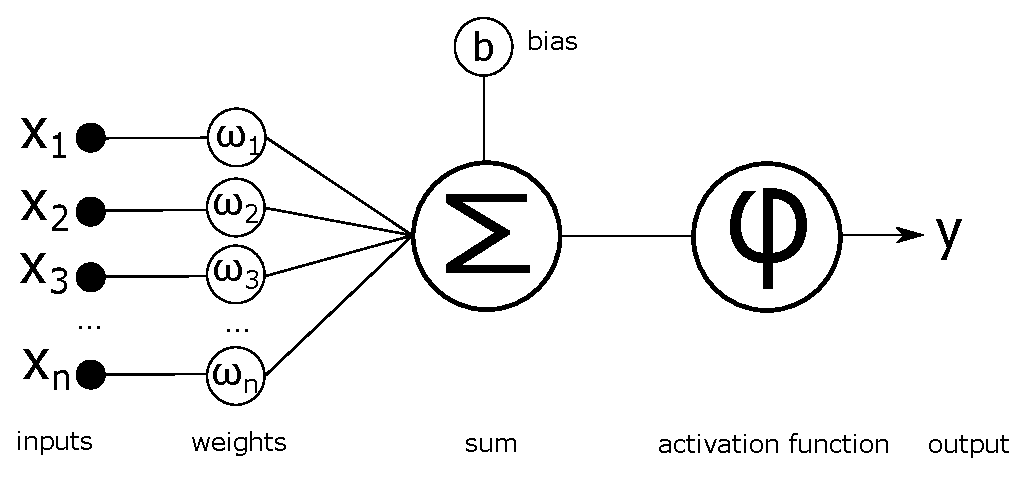
\includegraphics[width=10cm]{neuron.eps}
	\centering
	\caption{Symbolic structure of an artificial neuron.}
	\label{neuron_structure}
\end{figure}

\subsection{Layer}
\paragraph{}
Generally speaking, a layer represents an arbitrary transformation of input data inside the neural network. It is the essential building block of the neural network model in many deep learning frameworks (Tensorflow, Keras and et cetera). An organization of layers forms a computational graph defining operations performed on data. Layers do not even have to consist of any artificial neuron at all since a layer can be defined using other mathematical operation over the input data. However, the rest of this subsection is going to discuss a \textit{dense} layer, which is made up of the neurons introduced in section \ref{aritificial_neuron}.

\paragraph{}
When neurons are organized into the layer, it is not necessary to compute an output activation of each neuron one by one. Instead, the vector form of the equation for one neuron can be used to calculate the activation of the whole layer (equation \ref{layer_computation}). $W^T$ then denotes a transposed matrix of all the weights in the layer, $x$ is a vector of inputs and $b$ is a vector of biases \cite{Nielsen}. The function $\varphi$ is the activation function and is applied element-wise on the resulting vector $W^T x + b$. 

\begin{equation}
y = \varphi(W^T x + b)
\label{layer_computation}
\end{equation}  

Equation \ref{layer_computation_example} shows a detailed expansion of equation \ref{layer_computation} for a layer made up of two neurons and three inputs. In the expanded equation, $y_i$ denotes an output activation of the $i$-th neuron, $w_{ij}$ indicates a weight of the $j$-th input in the $i$-th neuron, $b_i$ is a bias of the $i$-th neuron and finally, $x_j$ represents a value of the $j$-th input \cite{Nielsen}. 

\begin{equation}
\begin{bmatrix}
y_1 \\
y_2
\end{bmatrix} =
\varphi(
\begin{bmatrix}
w_{11} & w_{12} & w_{13}\\
w_{21} & w_{22} & w_{23}
\end{bmatrix}
\begin{bmatrix}
x_1 \\
x_2 \\
x_3
\end{bmatrix} + 
\begin{bmatrix}
b_1 \\
b_2
\end{bmatrix}
)
\label{layer_computation_example}
\end{equation}  

\subsection{Model}
\paragraph{}
The way how different layers are organized and connected (figure \ref{nn_model}) is called a neural network model. Generally, a model consists of three parts - an input layer, hidden layers and an output layer. The input layer stands at the very beginning of the network and represents an entry point for data. If the input is an $N$-dimensional vector, then the input layer has $N$ neurons inside. Moreover, the first layer is simplified and does not perform any computation. The only thing done is that the output activation of each neuron is set to the value of the corresponding input ($y_i = x_i$). Subsequent layers (\textit{hidden layers}) perform the main part of the computation (section \ref{forwardpass}). Finally, activations in the output layer, which stands at the end of the model, are used to determine a resulting class (section \ref{forwardpass}). 

\begin{figure}[!h]
	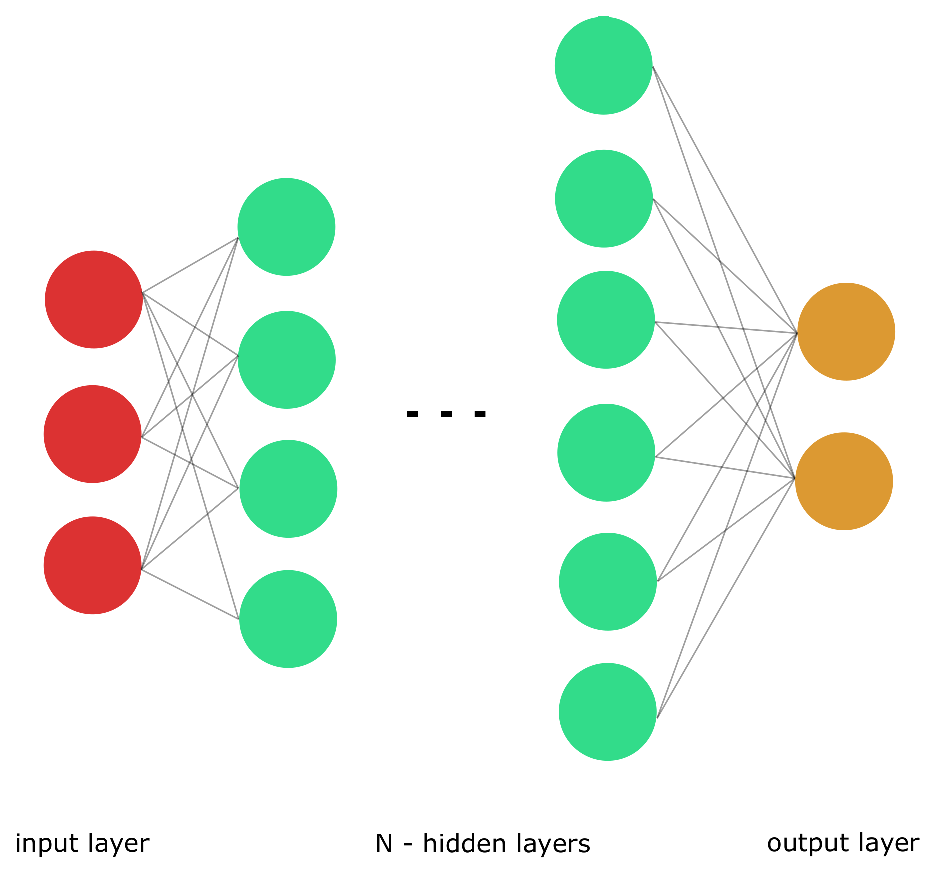
\includegraphics[width=10cm]{model.eps}
	\centering
	\caption{Example of a neural network model with four inputs, N hidden fully connected layers and two neurons at the output.}
	\label{nn_model}
\end{figure}

\section{Activation Functions}\label{activation_function}
\paragraph{}
An essential part of each neural network is a non-linear activation function, which is used to obtain the activation of a neuron/layer (equation \ref{neuron_computation}). Its most significant contribution is introducing a non-linearity into the model. Without such function, the neural network would be able to model only a linear dependency of a class on input data. It is because the output of the model would then consist of a linear combination of the input and the network parameters only \cite{deep_learning_with_python}.

\subsection{Sigmoid}
\paragraph{}
A sigmoid function (equation \ref{sigmoid_activation_eq}) is commonly used in output layers for tasks such as logistic regression or multi-label classification tasks. However, it is suitable for hidden layers as well \cite{python_ml_2nd}. Its major drawback is a vanishing gradient (draws near zero) for low and high values of the $z$. 

\begin{equation}
\varphi(z) = \frac{1}{1+e^{-z}}
\label{sigmoid_activation_eq}
\end{equation} 

\subsection{Hyperbolic Tangent (TanH)}
\paragraph{}
A hyperbolic tangent (equation \ref{tanh_activation_eq}) is similar to the sigmoid function in its shape and drawbacks, with the difference that a range of values is $<\!-1, 1\!>$, whereas sigmoid's range is $<\!0, 1\!>$. This activation function is predominantly used in hidden layers \cite{activation_functions_article}.

\begin{equation}
\varphi(z) = \frac{e^z - e^{-z}}{e^z + e^{-z}}
\label{tanh_activation_eq}
\end{equation} 

\subsection{Rectified Linear Unit (ReLU)}
\paragraph{}
A rectified linear unit is a straightforward activation function, which is defined as a maximum of zero and $z$. A significant advantage of ReLU is that it is computationally efficient and despite its simplicity, it turns out to work very well for a wide range of tasks. It is typically used in hidden layers \cite{python_ml_2nd}.

\begin{equation}
\varphi(z) = max(0, z)
\label{relu_activation_eq}
\end{equation} 

\subsection{Softmax}\label{softmax}
\paragraph{}
A softmax function (equation \ref{softmax_activation_eq})\cite{ml_probabilistic} is frequently used in output layers of the neural network thanks to its ability to transform the inputs into a probability distribution for the classes. It means that a sum of the softmax's output vector elements is always equal to one. In combination with a cross-entropy loss, it forces the network to give the highest predicted probability to the class given by the label and to assign as low probability as possible to the rest of them. 

\paragraph{}
It is worth mentioning that including the softmax in the activation functions section is questionable. It is due to the impossibility to compute an activation of a single neuron using the softmax. This fact can be seen in equation \ref{softmax_activation_eq}, where the knowledge of an inner product $z_j$ (bias added to the weighted sum) of all the neurons in the layer is necessary to scale the inner product of the current ($i$-th) neuron $z_i$. Therefore the softmax is often perceived as a self-standing softmax layer.

\begin{equation}
\varphi(z)_i = \frac{e^{z_i}}{\sum_{j=1}^{K} e^{z_j}}
\label{softmax_activation_eq}
\end{equation} 

\section{Classification Using a Neural Network}\label{forwardpass}
\paragraph{}
A classification task can be defined as a process of feeding in one sample of data, passing it through the whole model and determining the resulting class. This process is called a forwardpass and starts with setting output activations of neurons in the input layer according to values of the input. Then, the activation of the input layer is used as an input for the subsequent hidden layer. Generally, activation of the $n$-th layer is used as an input for the ($n+1$)-th layer. This step is done repeatedly until the output layer is reached.

\paragraph{}
Finally, when the activation of neurons in the output layer is known, a resulting class can be determined. Let us say that each neuron in the output layer represents one class, then a result of the classification is the one with the highest activation. 

\section{Loss/Cost Functions}\label{loss_function}
\paragraph{}
As further explained in section \ref{training}, the loss function is used during training as a measure of how good or bad the current setting of network parameters is. It should be noted that the value of the loss is not a suitable measure of a network accuracy. For this purpose, metrics introduced in section \ref{metrics} shall be used. Moreover, the selection of the loss function should be tailored to the metric we want to maximize, due to uncorrelation between some losses and metrics (section \ref{f1_loss}).

\subsection{Mean Squared Error}\label{MSE}
\paragraph{}
Mean squared error (MSE) is a loss function that is defined by equation \ref{MSE_eq} and suits well for regression tasks \cite{deep_learning_with_python}. In the equation, $C$ denotes the loss function, $w$ and $b$ are sets of all weights and biases of the neural network, respectively and $X$ is the current batch of inputs. On the right-hand side, there is a sum of the differences of labels $y$ and predicted values $\hat{y}$ summed over all inputs in the batch. Finally, the sum is divided by the number of examples $n$.

\begin{equation}
C(w, b, X) = \frac{1}{n}\sum_{x}^{} (y - \hat{y})^2
\label{MSE_eq}
\end{equation} 

\subsection{Cross-Entropy}\label{cross_entropy}
\paragraph{}
Another kind of a loss function is a cross-entropy loss (equation \ref{cross_entropy_eq}), which is often used for classification problems \cite{deep_learning_with_python}. The left side of the equation is identical to equation \ref{MSE_eq} and is described in section \ref{MSE}. On the right side, there is a negative-sum of product $y_{c}log(p_{c})$ over all possible classes $M$. In the product, $y_{c}$ is a binary class indicator - equal to 1 if the true class of a current sample is $c$, else 0. Finally $p_{c}$ is a probability of the current sample belonging to class $c$ \cite{cross_entropy}. Value of $p_{c}$ is determined by a softmax output layer (section \ref{softmax}) with which, the cross-entropy should be used.

\begin{equation}
C(w, b, X) = -\sum_{c=1}^{M} y_{c}log(p_{c})
\label{cross_entropy_eq}
\end{equation} 

\subsection{F1 Loss}\label{f1_loss}
\paragraph{}
In some cases, it might happen that the loss value does not correlate with a metric meant to be maximized. In other words, even if the loss decreases, the maximized metric may decrease as well. However, the expectation is that if we get better (lower) loss, we get a better (higher) value of the metric. This phenomenon can appear when the maximized metric is an f1 score (section \ref{f1_score}) and the chosen loss is a cross-entropy \cite{f1_loss}. In situations such as this, it is necessary to select another loss function, which can result in a better-trained model.

\paragraph{}
To maximize the f1 score (section \ref{f1_score}) it can be favorable to use the f1 loss. Equation \ref{f1_loss_eq} states how the f1 loss is calculated. The equation is the same as in the case of the f1 score. However, the meaning of $TP$ (true positives), $FP$ (false negatives), $FN$ (false negatives) is different from the f1 score. That is to be able to differentiate the loss. For example, if a label is $1$ and a model's prediction is $0.8$ probability for class $1$, we count $TP=0.8*1$, $FN=0.2*1$ and $FP=0.8*0$. Generally, this calculation is described by equations \ref{f1_loss_partials_eq} \cite{f1_loss_towards}.

\begin{equation}
C(w, b, X) = \frac{1}{n}\sum_{x}^{}(\frac{2TP}{2TP+FP+FN})
\label{f1_loss_eq}
\end{equation} 

\begin{equation}
\begin{gathered}
TP = prediction * label \\
FN = (1 - prediction)*label \\
FP = prediction * (1-label)
\label{f1_loss_partials_eq}
\end{gathered}
\end{equation} 

\section{Training a Neural Network Model}\label{training}
\paragraph{}
Thanks to equation \ref{layer_computation} and a description of the forwardpass in section \ref{forwardpass}, it shall be clear that a result of classification is a function of input values, weights and biases. Since the input values are fixed, the only way how to affect the behavior of a neural network model is to adjust the weights and biases. The weights and biases are called parameters of the network.

\paragraph{}
The process of setting the weights and biases (which may be randomly initialized at the begging) to maximize the accuracy of the network is called training. To measure how optimal our current setting is, we define a loss function (section \ref{loss_function}). A higher value of the loss means a worse accuracy of the network. In other words, we try to minimize the loss. However, the loss is a function of thousands of variables (mostly network parameters),
which is the reason why it is not possible to find optimal values for all the
parameters analytically. Due to that, an approximation of the loss minimum
has to be found using gradient optimization methods (see section \ref{optimizers} for details).

\paragraph{}
The training procedure (minimizing the loss) is described in the following steps, which are performed in a loop over all dataset batches \cite{deep_learning_with_python}:

\begin{enumerate}
	\item Select a batch of training examples from a training dataset.
	\item Do a forward pass with the selected examples and get predictions.
	\item Compute the value of a loss over the current batch using the obtained predictions and true labels.
	\item Compute an error of each neuron in an output layer using the loss.
	\item Propagate the error to previous layers (this process is called a backpropagation).
	\item Adjust parameter values to minimize the error (minimize the loss).
\end{enumerate}

The loop over all the batches is performed multiple times (\textit{epochs}). Since the previous steps are only a brief description of the training process, refer to the book by M. Nielsen \cite{Nielsen} for further details.

\subsection{Optimizer}\label{optimizers}
\paragraph{}
An optimizer represents an exact algorithm that is used for adjusting the network parameters \cite{deep_learning_with_python}. Generally, the optimization is based on computing a gradient (direction of the steepest increase) for each parameter with respect to the loss. The calculated gradient is used to move a value of the parameter against the gradient direction by a certain amount of the gradient's size. The amount of change is called a learning rate and is denoted as $\eta$. The learning rate is a member of a particular  group of parameters called hyperparameters. They represent network parameters that are not learned during the training.

\paragraph{}
Examples of commonly used optimizers are listed below:

\begin{itemize}
	\item Stochastic gradient descent (SGD) \cite{sgd}
	\item RMSProp \cite{RMSprop}
	\item AdaGrad \cite{adagrad_paper}
	\item Adam \cite{Adam_paper}
\end{itemize}

\section{Metrics}\label{metrics}
\paragraph{}
As stated in section \ref{loss_function}, a loss function is not the best for measuring how well a network is trained. For this purpose, it is necessary to use other metrics that are presented in this section.

\subsection{Accuracy}\label{accuracy}
\paragraph{}
Accuracy is defined as a fraction of correctly classified examples (equation \ref{accuracy_eq}). Even though this metric is the most often used one, it is not suitable for datasets with an unbalanced number of samples in the classes. For instance, if there is a binary classification task and we have a dataset with 95\% of "true" examples, the classifier can achieve a 95\% accuracy only by classifying all the data as "true". It means that it might be reasonable to use another metric, such as an f1 score (section \ref{f1_score}), that does not suffer from this drawback.

\begin{equation}
acc = \frac{\: correctly\: classified}{total\: number\: of\: examples}
\label{accuracy_eq}
\end{equation} 

\subsection{Precision, Recall and F1 score} \label{f1_score}
\paragraph{}
Before defining what a precision, recall and f1 score are, it is necessary to establish the concept of true positives (TP), true negatives (TN), false positives (FP) and false negatives (FN), which are possible results of a binary classification. Table \ref{result_classes_f1} states the individual cases and assigns a correct result class (TP, TN, FP, or FN) to them \cite{python_ml_2nd}. 

\begin{table}[h!]
	\centering
	\begin{tabular}{c c c} 
		\hline
		Label & Prediction & Result class \\ [0.5ex] 
		\hline\hline
		1 & 1 & TP \\ 
		1 & 0 & FN \\
		0 & 1 & FP \\
		0 & 0 & TN \\ [1ex] 
		\hline
	\end{tabular}
	\caption{Possible results of binary classification and underlying result classes.}
	\label{result_classes_f1}
\end{table}

\paragraph{}
Using the previously declared result classes, the precision, recall and the f1 score can be defined. The precision (equation \ref{precission_eq}) is a fraction of correctly classified positive samples from all samples classified as positive (equation \ref{recall_eq}). The recall is a fraction of correctly classified positive samples from all the truly positive samples. Finally, the f1 score is defined as  a harmonic mean of precision and recall (equation \ref{f1_score_eq}). As stated in section \ref{accuracy}, the f1 score is extremely useful for the evaluation on unbalanced datasets. 

\begin{equation}
precision = \frac{TP}{TP + FP}
\label{precission_eq}
\end{equation} 

\begin{equation}
recall = \frac{TP}{TP + FN}
\label{recall_eq}
\end{equation} 

\begin{equation}
f1\_score = 2\:\frac{precission*recall}{precission+recall}
\label{f1_score_eq}
\end{equation} 

\paragraph{}
Even though the stated computation works for binary classification only, there are three possible ways of how to generalize the f1 score for multi-class classification. This generalization can be made using a micro, macro and weighted f1 score \cite{multiclass_f1_score}.

\subsection{Confusion Matrix}
\paragraph{}
A confusion matrix (figure \ref{conf_matrix_example}) is a handy metric for evaluating network behavior in detail. Its significant benefit is that it shows which classes are being confused during the classification. It means that the confusion matrix is a $C \times C$ sized matrix where each member $n_{ij}$ of the matrix denotes the number of cases when a sample of the $i$-th class was classified as the class $j$. Thanks to that, we can identify classes that the model struggles to distinguish the most. The confusion matrix may also appear in a normalized form, where each row is normalized to one.

\begin{figure}[!h]
	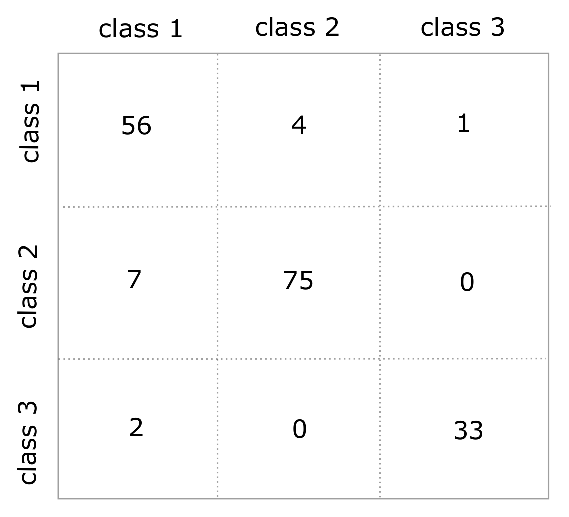
\includegraphics[width=7cm]{conf_matrix.eps}
	\centering
	\caption{An example of a confusion matrix for three-class classification. For example, it shows that a sample from class 2 was classified as a class 1 for seven times.}
	\label{conf_matrix_example}
\end{figure}

\section{Other Neural Network Concepts and Techniques}\label{other_nn_architectrues_and_techniques}
\paragraph{}
A concept of the multilayer perceptron does not suit very well for all tasks where neural networks can be utilized. Therefore, many other architectures dealing with different drawbacks of the original concept were developed. One such architecture, which tries to address a problem of multi layer perceptron's inability to deal with sequential data, is a recurrent neural network (RNN) \cite{RNN_LSTM} and its often used bi-directional form \cite{RNN_LSTM}. An extension of this concept is a gated recurrent unit (GRU) and a long short term memory (LSTM)\cite{colahs_lstm} network that can handle long term dependencies in the sequences. The concept of RNNs is often amended by an attention mechanism  \cite{colahs_attention}.

\paragraph{}
Another type of architecture is a convolutional neural network (CNN), which applies a convolution operation over a sliding window to discover patterns emerging in the input \cite{python_ml_2nd}. This concept is often used for image or video classification and natural language processing. 

\paragraph{}
Although these concepts are quite diverse, they all suffer from a common problem, which is overfitting \cite{Nielsen}. This phenomenon can be identified by achieving perfect training accuracy while having poor results on a validation part of the dataset. To cut down the influence of the overfitting, regularization techniques can be used. An example of a regularization technique is an L2 regularization \cite{Nielsen} or a dropout \cite{droupout_in_cnns}.

\subsection{Siamese Neural Networks}
\paragraph{}
The previously discussed multilayer perceptron can be perceived as a sequential network (figure \ref{sequential_neural_network}), since layers are organized into an ordered sequence that defines the flow of computation. However, the sequential network that accepts one input vector (or one sequence) is not the only type of neural network architecture. 

\begin{figure}[!h]
	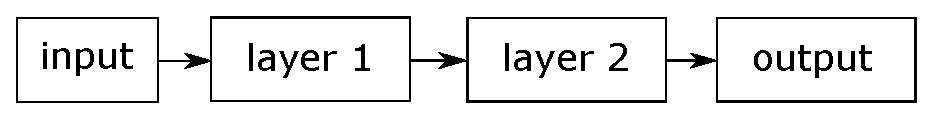
\includegraphics[width=13cm]{sequential_nn.eps}
	\centering
	\caption{An example of a sequential neural network.}
	\label{sequential_neural_network}
\end{figure}

Generally, the neural networks can have multiple input vectors or sequences and the organization of the layers can be diverse. A special type of architecture is a siamese network \cite{siamese_nn}. This kind of network accepts two inputs that are passed through two parallel subnets sharing their weights. The two subnets can be followed by other layers processing an output of the subnets. An example of siamese network architecture is depicted in figure \ref{siamese_neural_network_fig}. Such architecture finds its usage, for example, in facial recognition or semantic similarity (section \ref{semantic_similarity_tasks}).

\begin{figure}[!h]
	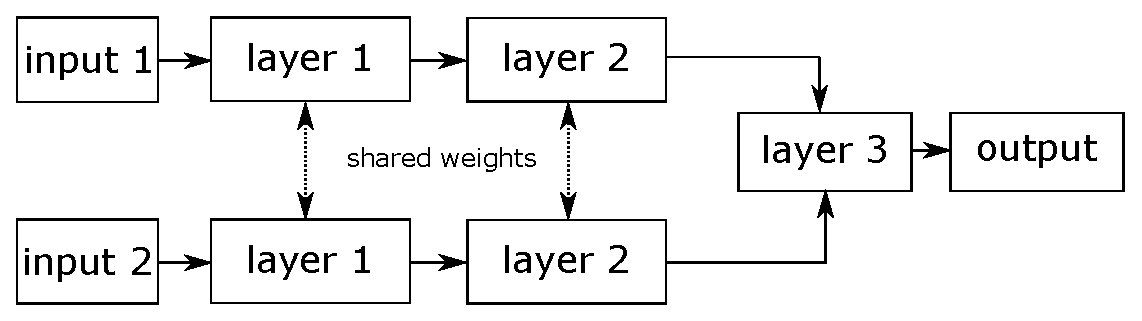
\includegraphics[width=13cm]{siamese_nn_overall.eps}
	\centering
	\caption{A siamese neural network that accepts two inputs and produces one output vector. The layers on the same level share their weights, as marked in the picture.}
	\label{siamese_neural_network_fig}
\end{figure}  



\chapter{Semantic Vector Representation of Text}\label{vector_repr_chapter}
\paragraph{}
A natural language processing (NLP) is a subfield of linguistics and computer science. In recent years many deep learning techniques have been successfully applied to many NLP problems. These are, for instance, sentiment analysis, machine translation, text classification, semantic similarity and many more \cite{nlp_devopedia}. 

\paragraph{}
A problem in the NLP is that a dimension of the space of possible words or sentences fed into a neural network is immensely high. The way how neural networks deal with it is that each subsequent layer creates more abstract and usually lower-dimensional features from the one created by the previous layer. Figure \ref{embedding_dim_red_figure} shows such a hierarchy, where the words are fed into a neural network as a one-hot representation. Then, subsequent layers create more abstract features, which can be perceived as word embeddings, sentence embeddings, higher-level features and finally, as a vector determining the resulting class.

\begin{figure}[!h]
	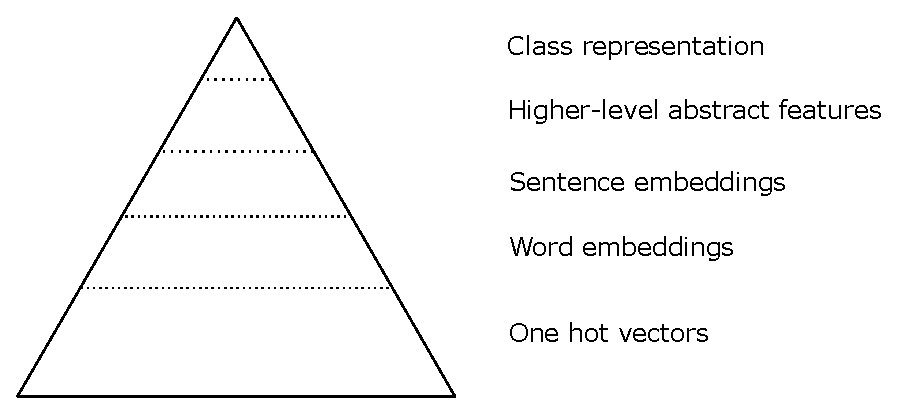
\includegraphics[width=13cm]{embedding_dim_red.eps}
	\centering
	\caption{A pyramid of abstraction of processing a natural language using neural networks}
	\label{embedding_dim_red_figure}
\end{figure}

\paragraph{}
In some cases, it might be beneficial to pre-train a part of the neural network in advance. For example, it is possible to pre-train word embeddings or a whole sentence encoder that is later used to build the final neural network. The pre-training can be done in a supervised as well as unsupervised way.

\section{Vector Representation of Words}\label{word_embedding}
\paragraph{}
An embedding of words can be directly useful for a lot of NLP tasks. Moreover, since sentences are made up of words, text representation techniques are often based on the word embeddings. The desired word representation is a low dimensional vector (about hundreds of dimensions) of real numbers that captures the semantics of the word. Put differently, it is expected that two similar words appear close to each other in a vector space of the representations. A favorable fact is that the embeddings can be trained using unsupervised learning on a large text corpus. Such techniques are usually based on a distributional hypothesis \cite{nlp_eisenstein}.

\paragraph{}
In this section, two types of word representations - context-free and contextual representations are presented. At the end of the section, a concept of subword models is also briefly discussed.

\subsection{Context-Free Word Representation}\label{context_free_embedding}
\paragraph{}
Context-free word representation techniques are identified by creating a fixed vector for each word, no matter its context. It means that, for example, the word "bank" would have the same representation when it appears in a context "bank account" as in case it appears in a context "river bank" \cite{bert_ithub}.

\paragraph{}
An advantage of this approach is that unlike the contextual representations, the word embedding is self-standing. Therefore, a similarity score of two words can be computed and used for similar word search.

\subsubsection{Word2Vec}\label{w2v}
\paragraph{}
A Word2Vec \cite{word2vec} is an unsupervised technique to represent words as vectors. Generally, this algorithm can be found in two forms. The first one is called a continuous bag of words (CBOW) and lies in predicting a target word given its context. The other method, on the contrary, predicts the context given a central word and is known as a skip-gram model. 

\paragraph{}
The skip-gram model is trained in a way that the central word is used as an input to a neural network that produces a conditional probability of the central word co-occurring next to other adjacent words in a sliding window. The window size defines the number of neighboring words taken into account. Then the vector representing the central word (which is stored in a weight matrix of the network) is adjusted to maximize the computed conditional probabilities for the neighboring words. The way how the CBOW model is trained is analogical and further explained in \cite{training_word2vec} together with mathematical details of the skip-gram model.

\subsubsection{Global Vectors (GloVe)}
\paragraph{}
Global Vectors (GloVe) \cite{glove} are another method of creating word embeddings. Unlike Word2Vec, GloVe utilizes a global word co-occurrence statistic that is captured in a co-occurrence matrix. To turn such a matrix into a vector representation, the authors introduced a new algorithm. It is based on optimizing the word vectors so that the dot product of the two word embeddings is equal to a logarithm of their co-occurrence count.

\subsection{Contextual Word Representation}
\paragraph{}
As stated in section \ref{context_free_embedding}, the context-free representations do not capture the context in which a word is used and this feature may be undesirable in many NLP tasks. Fortunately, contextual word representation techniques exist. The idea is that hidden layers in an LSTM based language model contain contextualized representations of fed-in words. The usage of such embeddings is then different than with the fixed representations, such as pre-trained Word2Vec (section \ref{w2v}). Instead of querying a lookup table, the vector embedding is obtained by passing the words into a model that produces the contextual embedding later used as an input to a task-specific neural network. An example of contextual word representations based on the deep bi-directional LSTM language model is ELMo (Embeddings from Language Models) \cite{elmo}.

\paragraph{}
Another contextual embedding method is a BERT \cite{bert} (Bidirectional Encoder Representations from Transformer) model. This model is based on Transformer architecture \cite{attention_is_all_you_need}, and its utilization provides outstanding results in many tasks.

\subsection{Subword Embedding}\label{subword_models}
\paragraph{}
A significant drawback of the techniques presented in section \ref{context_free_embedding} is that they are not able to handle uncommon and out of vocabulary words (OOVs) - word for which an embedding does not exist. Techniques trying to overcome this obstacle are called subword embeddings and are based on dividing words into smaller units down to a character level. For instance, the word "inevitable" can be composed of two units "in" and "evitable".

\subsubsection{Byte-Pair Encoding}\label{BPE}
\paragraph{}
A byte-Pair encoding \cite{nlp_stanford} is an unsupervised text segmentation algorithm which originated as a compression method. The algorithm starts with a list of elementary symbols, such as characters. Then it creates a new symbol composed of the most frequent symbol pair that appears in the training text. This step is repeated until the desired size of the vocabulary is achieved.

\subsubsection{WordPiece}
\paragraph{}
Another unsupervised method for subword tokenization is a WordPiece algorithm \cite{nlp_stanford}, which is to some extent similar to the Byte-Pair encoding (section \ref{BPE}). The difference is in the merging step. Instead of combining the two most frequent pairs, WordPiece chooses a couple, that would increase the log-likelihood of a language model \cite{nlp_eisenstein} if added to the vocabulary.

\section{Vector Representation of Sentences}\label{vector_representation_of_sentences}
\paragraph{}
As stated in the introduction of chapter \ref{vector_repr_chapter}, having a robust vector representation of text may be advantageous or even necessary for many NLP tasks. In this section, some of the used methods for obtaining semantic sentence embeddings are presented. 

\subsection{Combining Word Embeddings}\label{word_averaging}
\paragraph{}
Simple methods obtain a vector representation of text by combining pre-trained word vectors. One way how to combine the word embeddings is a summation or a weighted average, where the weights are tf-idf scores computed from a language corpus \cite{weighted_averaging_tfidf}. The tf-idf score for the $i$-th word is calculated according to equation \ref{tf_idf_eq}, where $k$ is the number of all words in the $j$-th document and $n_{xy}$ denotes an occurrence count of the $x$-th word in the $y$-th document. Finally $|D|$ is the number of documents in the corpora and  $|\{j:t_i \in d_j\}|$ is the number of documents where the word $i$ appears.

\begin{equation}
tf\_idf_i = \frac{n_{ij}}{\sum_{k}n_{kj}} * log \frac{|D|}{|\{j:t_i \in d_j\}|}
\label{tf_idf_eq}
\end{equation}  

\subsection{Supervised Representation Learning}\label{supervised_repre_learning}
\paragraph{}
A different way how to get a robust vector representation of text is to train a neural network model on a supervised learning task since the sentence embedding would then lie in hidden layers of the neural network. For example, in case of a network that consists of an embedding layer on the beginning, two LSTMs above it and two dense layers at the output, the representation of the sentence can be taken from the output of the second LSTM layer. A significant downturn of this method is a necessity of a labeled dataset that may not be available in many cases.

\paragraph{}
The quality of the embeddings obtained by this technique depends on the choice of a learning objective. Examples of such tasks are, for instance, machine translation or natural language entailment (section \ref{snli}). Another supervised learning objective is a semantic similarity task, which aims to recognize whether two texts are similar or not on a semantic basis. This task is going to be further focused by the rest of the work and a more detailed description can be found in section \ref{semantic_similarity_tasks}.

\subsection{Unsupervised Representation Learning}
\paragraph{}
In cases when a labeled dataset is not available, an unsupervised representation learning might come into play. Generally, a principle of the supervised representation learning (section \ref{supervised_repre_learning}) applies for the unsupervised case in the same way - the desired vector representation of sentences is in the hidden layers. The difference is the choice of the learning task, which is unsupervised in this case. 

\paragraph{}
To give an example, the BERT model \cite{bert} is trained on two unsupervised tasks. The first one is to predict a randomly masked token from an input sequence based on its context. The second one is the next sentence task, which aims to predict whether one sentence follows the other one in the original text. Another unsupervised learning model called GPT-2 \cite{GPT2} is trained on predicting the next word in a text.

\section{Semantic Similarity Task}\label{semantic_similarity_tasks}
\paragraph{}
In many real applications of the NLP, such as search engines, it is essential to measure or identify whether two texts are similar or not. Although this may look easy to accomplish just by looking if both documents contain the same keywords, distinguishing between tiny semantic nuances may be a severe problem. To differentiate texts with minor semantic differences is a target of a semantic similarity task, which is under ongoing research at the moment. Generally, the approach is to embed sentences into an $n$-dimensional space and then to compute a cosine similarity (equation \ref{cosine_similarity_eq}) or another metric of the two vectors. 

\begin{equation}
similarity = cos(\theta) = \frac{A \cdot B}{||A|| \: ||B||}
\label{cosine_similarity_eq}
\end{equation}

\paragraph{}
Therefore, the main objective of the semantic similarity task is to create embedding vectors that contain robust semantic information (section \ref{vector_representation_of_sentences}). The following sections present the related datasets and techniques.

\subsection{Related Datasets}\label{semantic_similarity_datasets}
\paragraph{}
For the semantic similarity task, there is not a lot of data available, which is a crucial problem in this field. While some datasets suffer from a small size, some of the others are partially made up of automatically generated samples, which may be undesirable as well. In this section, some of the available datasets are discussed.

\subsubsection{STS Benchmark}
\paragraph{}
STS benchmark dataset \cite{STSbenchmark} is a subset of data used in SemEval competitions. Examples contained in the dataset come from various sources such as user forums, image captions and news headlines. The dataset is separated into three subsets - training, development and testing. The total size of the dataset is around 8 600 samples and the sizes of the dataset parts are shown in table \ref{STSbenchmark_counts}.

\begin{table}[h!]
	\begin{center}
		\begin{tabular}{l r} 
			\hline
			\textbf{Dataset part} & \textbf{Dataset size} \\ [0.5ex] 
			\hline\hline
			training & 5 749 \\ 
			development & 1 500 \\
			testing & 1 379 \\ 
			\hline
		\end{tabular}
	\end{center}
	\caption{Sizes of training, development and testing parts of the STS Benchmark dataset.}
	\label{STSbenchmark_counts}
\end{table}

\subsubsection{Stanford Natural Language Inference Dataset}\label{snli}
\paragraph{}
A Stanford Natural Language Inference dataset (SNLI) \cite{snli} consists of human-labeled pairs of sentences. The possible labels are a contradiction, entailment, and neutral relationship. Although a learning objective of this dataset is not the semantic similarity, a natural language inference task requires a meaningful vector representation of sentences in the same way as the semantic similarity does. In other words, the significant difference lies in the classifier built over the representations. Thanks to that, the SNLI can be used for both an evaluation and training of the semantic representations of a text. 

\paragraph{}
The SNLI dataset, which consists of 570 000 examples, is split into three parts - training, development and testing. The sizes of these parts are shown in table \ref{SNLI_counts}. The amount of data and a lack of automatically generated examples make SNLI a very reasonable choice for many researchers. An example of the dataset pairs with the corresponding labels from the original paper \cite{snli} are shown in table \ref{SNLI_examples}.

\begin{table}[h!]
\begin{center}
	\begin{tabular}{l r} 
		\hline
		\textbf{Dataset part} & \textbf{Dataset size} \\ [0.5ex] 
		\hline\hline
		training & 550 152 \\ 
		development & 10 000 \\
		testing & 10 000 \\ 
		\hline
	\end{tabular}
\end{center}
\caption{Sizes of training, development and testing parts of the SNLI dataset.}
\label{SNLI_counts}
\end{table}

\begin{table}[h!]
	\begin{center}
		\begin{tabular}{p{5cm} p{5cm} p{2cm}} 
			\hline
			\textbf{Text} & \textbf{Hypothesis} & \textbf{Label} \\ [0.5ex] 
			\hline\hline
			A man inspects the uniform of a figure in some East Asian country. & The man is sleeping. & contradiction \\ 
			\hline
			An older and younger man smiling. & Two men are smiling and laughing at the cats playing on the floor. & neutral \\
			\hline
			A soccer game with multiple males playing. & Some men are playing a sport. & entailment \\ 
			\hline
		\end{tabular}
	\end{center}
	\caption{Three examples from the SNLI dataset.}
	\label{SNLI_examples}
\end{table}

\subsection{Related Work}\label{semantic_similarity_related_work}
\paragraph{}
Since the rest of the work focuses on the vector representation of text enriched with source code snippets, the following section presents an existing work on related topics. The paragraphs provide a brief description of the papers. A more detailed description can be found in the cited sources.

\subsubsection{A large annotated corpus for learning natural language inference}
\paragraph{}
Authors of the SNLI dataset published the results of three different models in their paper \cite{snli}. Generally, all of their models consist of a word embedding layer for both premise and hypothesis and a sentence embedding layers on the top of the word embeddings. In the end, classification is done by three 200-dimensional dense layers taking the 100-dimensional representation of the premise and hypothesis as an input. At the output, there is a softmax layer. A difference between these models is a method of sentence representation. The first and most simple model uses a sum of the word embeddings. The next one uses a simple RNN layer, whereas the last one uses an LSTM layer for sentence representation. The latest mentioned model is the most successful one with a test accuracy of $77.6\%$.

\subsubsection{Shortcut-Stacked Sentence Encoders for Multi-Domain Inference}
\paragraph{}
In 2017, Nie X. and Bansal M. presented their work on a Shortcut-Stacked Sentence Encoder \cite{shortcut_stacked_sentence_encoders}. It aims to represent a sentence as a vector of real numbers that is later used for an NLI classification. The model is made up of three bi-directional LSTM layers with shortcut connections and a classifier on top of it. The shortcut connections are made in the way that input of each LSTM layer consists of an original word embedding concatenated with a corresponding sequential output of all the preceding LSTMs. Such an approach led to an $86.0\%$ accuracy on the SNLI dataset.

\subsubsection{Sentence Embeddings in NLI with Iterative Refinement Encoders}
\paragraph{}
Another work \cite{HBMP} related to obtaining a vector representation of text introduces a hierarchical structure of bi-directional LSTM layers that implements an iterative reinforcement strategy. The key idea behind the model is that each subsequent LSTM layer is initialized with the last hidden state of the preceding layer while accepting the original word embeddings as an input. An output of each LSTM is then max-pooled and concatenated to a resulting representation. The authors have reported a very good accuracy of $86.6\%$ on the SNLI dataset.


\subsubsection{Dynamic Self-Attention Model}
\paragraph{}
Yoon D., Lee D. and Lee S. in their paper \cite{DSA} presented a new Dynamic Self-Attention (DSA) model, which outperforms many related models. DSA is based on attending to a dynamic weight vector rather than to a fixed vector learned during training. The model succeeded on the SNLI dataset with a result of $87.4\%$, which is the highest score among reported results in a sentence vector-based group of models.

\subsubsection{Semantics-aware BERT for Language Understanding}
\paragraph{}
At the moment, the best reported result on the SNLI dataset is achieved by a model called Semantic-aware BERT (SemBERT) \cite{semBERT}. It is a BERT \cite{bert} model extended by information about a semantic role of different parts of an input. More precisely, the BERT model is used to compute a contextual representation of word tokens. It is then concatenated with a vector, which carries the information about the semantic role of the token in a particular sentence. An achieved accuracy on the SNLI dataset is $91.9\%$.
 
\subsubsection{Retrieval on Source Code: A Neural Code Search}
\paragraph{}
In their paper, Sachdev S. et al. \cite{facebook0_unsupervised} addresses a natural language search over a large code base acquired from the GitHub. They use a variant of a Word2Vec embedding (section \ref{w2v}) to obtain a representation of the query and a code snippet. Three methods of creating a document embedding based on the word representations are evaluated. These are simple averaging of all the word vectors, averaging unique words only and a weighted average using the tf-idf (equation \ref{tf_idf_eq}). Such embedding of the query is then used to find a code snippet with its representation closest to the query embedding. The accuracy of the code search was evaluated on 100 hand-picked StackOverflow questions with an accepted answer. The most promising result is achieved using the weighted average method, where an acceptable solution was found for 43 out of 100 test queries.

\subsubsection{When Deep Learning Met Code Search}
\paragraph{}
Another existing work \cite{facebook1_supervised} extends the previously discussed method by introducing supervision into the training. A significant difference is that the authors use two different embedding matrices (the first one is used for the code and the second for the query), initialized by the same pre-trained weights. These matrices are then fine-tuned during the training process. Additionally, the scheme of producing a document level embedding from the word token embeddings is changed. Instead of the tf-idf weighted average, a simple average is used for the query and a weighted average based on learned attention weights is used for the code. 


\chapter{Stackoverflow Data}\label{dataset}
\paragraph{}
A Stackoverflow is one of Stackexchange's community platforms, which is designated for programmers. It provides a space to ask questions and get answers from other members of the community. At the beginning of July 2019, the page contained more than 45 million questions and answers, which makes the Stackoverflow being considered as the biggest programming discussion platform.

\paragraph{}
Not only does the Stackoverflow store an enormous knowledge base, but the site also hides valuable hand-tagged data that can be used for machine learning. More precisely, users can mark two questions as duplicates so that it warns the others that there may be a desired solution already available. However, the interesting part thereof are the duplicate links themself. Thanks to them, the Stack Overflow data can be used to create a dataset for the semantic similarity task (section \ref{semantic_similarity_tasks}). Utilization of the duplicates for learning a sentence encoding is an aim of this work and will be focused in the subsequent chapters.

\paragraph{}
This chapter is structured as follows. Firstly a detailed description of the data source is given. Later the chapter discusses the structure of the data dump and presents essential data statistics. Finally, a short discussion about alternative data sources takes its place.  

\section{Data Source}
\paragraph{}

The export of the complete Stackoverflow website is available at \url{www.archive.org/details/stackexchange}. The work uses a page dump from the beginning of July 2019. Therefore the information stated by this work is related to this date. The export comes logically separated in eight compressed XML files, each carrying different information. The individual parts and their sizes (compressed) are listed below:

\begin{itemize}
	\setlength\itemsep{0.03em}
	\item badges (242.7 MB) - gained honors
	\item comments (4.2 GB) - user comments
	\item post history (25.0 GB) - history of posts
	\item \textbf{post links} (84.7 MB) - relationship links between the posts
	\item \textbf{posts} (14.3 GB) - all questions and answers
	\item tags (797.9 KB) - tags that can be associated with the posts
	\item users (504.8 MB) - profiles of page users
	\item votes (1.1 GB) - votes for the posts
\end{itemize} 

Only the post links and posts (both outlined using a bold font in the listing) thereof are used for assembling the dataset. A detailed description of the export parts relevant to the dataset is provided in the following section.

\section{Data Dump Structure}
\paragraph{}
As stated in the previous section, the Stackoverflow dump comes in XML files. Since not all the fields available in the XML are necessary, only the relevant ones are chosen to be further processed. A field listing of the posts and post links exports with the selected fields highlighted can be found below:

\begin{Verbatim}[commandchars=\\\{\},codes={\catcode`$=3\catcode`_=8}]
\textbf{posts.xml}
	\textit{\textbf{- Id}}
	\textit{\textbf{- PostTypeId    }  }  	
		-> 1: Question
		-> 2: Answer
	- ParentID (only present if PostTypeId is 2)
	- AcceptedAnswerId (only present if PostTypeId is 1)
	- CreationDate
	- Score
	- ViewCount
	\textit{\textbf{- Body}}
	- OwnerUserId
	- LastEditorUserId
	- LastEditorDisplayName
	- LastEditDate
	- LastActivityDate
	- CommunityOwnedDate
	- ClosedDate
	\textit{\textbf{- Title}}
	- Tags
	- AnswerCount
	- CommentCount
	- FavoriteCounts
\end{Verbatim}

\begin{Verbatim}[commandchars=\\\{\},codes={\catcode`$=3\catcode`_=8}]
\textbf{postlinks.xml}
	\textit{\textbf{- Id}}
	\textit{\textbf{- CreationDate}}
	\textit{\textbf{- PostId}}
	\textit{\textbf{- RelatedPostId}}
	\textit{\textbf{- PostLinkTypeId}}
		-> 1: Linked
		-> 3: Duplicate
\end{Verbatim}

From the listing above, it can be seen that the linking of the duplicates is done using a post link record with $PostLinkTypeID = 3$. Each post link has its unique identifier (\textit{Id}) and is assigned to one of the related posts via a unique identifier of the post (\textit{PostId}). The second post in the relationship is also determined by its identifier (\textit{RelatedPostId}). 

\paragraph{}
From the post attributes, the most important fields are \textit{Id}, \textit{PostTypeId}, \textit{Body} and the \textit{Title}. Worth mentioning is that the \textit{Body} attribute contains a formatted content of the post in an HTML.

\section{Data Statistics}
\paragraph{}
Table \ref{data_source_counts_analysis} shows document counts in different categories of the data. The first four of them are basic categories defined by a separation of the data source. The last four of them (separated by a horizontal line) are derived categories that are subsets of the posts.

\paragraph{}
From the table, it can be seen that the overall number of posts is around 45 million. 17.8 million of thereof are the questions, which are the point of interest in this work. Moreover, around 491 thousands of pairs of questions are the duplicates that will form a basis of the entire dataset. Another significant property observed in the data is that $76.6\%$ of the questions contain a code snippet (body of the post contains an HTML tag "<code>").

\begin{table}[h!]
	\begin{center}
		\begin{tabular}{l r} 
			\hline
			\textbf{Dataset part} & \textbf{Number of samples} \\ [0.5ex] 
			\hline\hline
			comments & 74 003 667 \\ 
			users & 10 640 388 \\ 
			post links & 5 600 831 \\ 
			posts & 45 069 473 \\
			\hline
			questions & 17 786 242 \\
			questions containing a code snippet & 13 628 089 \\
			questions with an accepted answer & 9 362 222 \\
			duplicate pairs of questions & 491 337 \\
			\hline
		\end{tabular}
	\end{center}
	\caption{Example counts in different document categories in the Stackoverflow data dump. Below the horizontal divider are derived categories that are subsets of the "posts" category.}
	\label{data_source_counts_analysis}
\end{table}

\section{Other Data Sources}
\paragraph{}
Besides the Stackoverflow duplicate questions, other data sources exist as well. One of the alternative data sources can be even obtained from the Stackoverflow dump by extracting pairs made up of questions and their corresponding accepted answers. The idea behind that is to use the accepted answers to predict whether the post is an answer to the given question.

\paragraph{}
Alternatively, the size of the current dataset might be enlarged with data from the remaining 173 webpages of the Stackexchange platform. That would bring more complexity into the dataset since each page focuses on a different topic such as 3D printing or math. Furthermore, variants of few Stackexchange pages exist in languages other than English.

\paragraph{}
Apart from the Stackexchange, there are other similar web pages, such as Quora. That page was already utilized to create a Quora Question Pairs dataset consisting of approximately 404 thousands of training examples. A training objective of the dataset is to predict whether two questions are duplicates or not. The dataset can be accessed on \url{https://www.kaggle.com/c/quora-question-pairs}.

\chapter{Analysis of the Problem}\label{analysis}
\paragraph{}
This work aims to create a sentence encoder using the dataset from Stackoverflow duplicate questions (chapter \ref{dataset}). Therefore, this work utilizes deep learning techniques to train a classifier distinguishing between different, similar (only some of the presented models) or duplicate questions. This chapter presents possible solutions for different sub-problems and discusses the chosen approaches.

\section{Assembling the Dataset}\label{assembling_the_dataset}
\paragraph{}
The first step in training a neural network is to obtain a dataset. To solve the given task, this work chooses to utilize duplicate questions obtained from the Stackoverflow webpage (chapter \ref{dataset}). The Stackoveflow page was chosen from the Stackexchange pages since it is the largest one. Additionally, it requires to address the domain specific language containing code snippets.

\paragraph{}
To assemble the dataset, it is essential to clean the data source. In this case, the data contain duplicate links pointing to a not existing post (the previously stated number of duplicates is after cleaning the invalid links).  That can be achieved by iterating over all the links and querying referenced posts. If one of the referenced posts cannot be found, the corresponding link is removed. All the remaining links are then used as a base for the dataset.

\paragraph{}
Generally, the learning objective of the created dataset shall be to classify whether two questions are duplicates or not. It implies that each example in the dataset is a triplet "(\textit{master post}, \textit{related post}, \textit{class})", where the class denotes the relationship between the two posts. Since the neural network must distinguish a tiny semantic difference in the questions, the dataset shall not consist of duplicates and different question pairs only. Therefore, the dataset must embrace similar question pairs as well. This work defines a question pair as similar if there is no duplicate link between the questions, but a keyword-based search query finds a match between them. Consequently, the dataset is made up of pairs of questions classified into the following categories: \textit{different}, \textit{similar} and \textit{duplicates}.

\paragraph{}
To assemble the dataset, firstly, the duplicates are found and assigned to each other. The process is to iterate over all the duplicate links and query the first post of the current link. This post is marked as a \textit{master post}. After that, all duplicates for the given \textit{master post} that are not already in the dataset are found. During the duplicate search, the links are handled transitively up to a depth of five links. Handling the links transitively may result in marking two questions as duplicates even though they are different (in case of the transitive links of a higher order). However, table \ref{transitive_duplicates} shows that transitive duplicates of higher order are not represented in the dataset in significant numbers. All the found duplicates are the assigned to the \textit{master post} and they are marked as \textit{duplicates}.

\begin{table}[h!]
	\begin{center}
		\begin{tabular}{l r r} 
			\hline
			\textbf{Relation type} & \textbf{Total examples} & \textbf{Percentage} \\ [0.5ex] 
			\hline\hline
			direct & 222 656 & 98.48\% \\
			1st transitive  & 3 226 & 1.43\% \\
			2nd transitive & 133 & 0.06\%  \\
			3rd transitive & 28 & 0.01\%  \\
			4th transitive & 25 & 0.01\%  \\
			5th transitive & 22 & 0.01\%  \\
			\hline
		\end{tabular}
	\end{center}
	\caption{Summary of duplicate examples obtained from direct links and transitive relations.}
	\label{transitive_duplicates}
\end{table}

\paragraph{}
After that, three similar posts that are not already in use shall be found for each \textit{master post} in the dataset. To perform such queries over the data, they must be stored in a database providing such functionality. Currently, there are many software tools for data storage, analysis and search available on the market. Examples of such databases are, for example, MySQL, MongoDB, Elastic stack, et cetera. This work chooses to work with the Elastic stack (Elasticsearch + Kibana) since it comes in a free, open-source version and provides suitable functions for data indexing, searching, exploration and visualization. The posts found using the Elasticsearch are assigned to the \textit{master post} and marked as \textit{similar}.

\paragraph{}
In the end, three randomly chosen posts (that are not in use already) are assigned to each of the master posts as a \textit{different} post. The different posts are chosen randomly since there is little likelihood that the post would be similar.

\section{Framework}
\paragraph{}
One of the essential decisions when it comes to neural networks is a framework choice. These days, many machine learning frameworks are available and each has its advantages and disadvantages. These are, for example, PyTorch, Scikit-learn, Tensorflow (TF), or Keras.

\paragraph{}
This work chooses to work with the Tensorflow 2.0 in combination with the in-built Keras. Together they provide extensive options to build, train and evaluate a neural network. Other significant advantages of the TF are the detailed tutorials that are freely available. Additionally, there is an active community that stands behind the TF. Moreover, a web application called Tensorboard can be used to display a computational graph of the network, view the training and evaluation results, or analyze how does a hyperparameter setup affects the resulting accuracy.

\section{Feeding the Data into a Neural Network}
\paragraph{}
Feeding dataset examples into a neural network for a purpose of training or evaluation requires to build an input pipeline. Its role is to load, shuffle and batch the examples. Furthermore, the raw data needs to be preprocessed before being ingested by the network. These points are discussed in detail in this section. 

\subsection{Input Pipeline}\label{input_pipelines}
\paragraph{}
The design of an input pipeline heavily depends on the features provided by the chosen framework. The Tensorflow provides a wide range of possibilities of feeding in the data. The first one is to build a complete instance of a TF Dataset class, which provides functionality to download, split and feed the data into the network. However, this approach is quite labor-intensive. That may be undesirable in the early phases of development since there is a chance that there will be additional changes in the dataset.

\paragraph{}
Another feasible approach is to omit the Dataset API entirely  and to use pure Python generators. Unfortunately, this results in losing a lot of useful functions that the API provides. A good compromise between implementation complexity and the features provided by the TF is to create an instance of a Dataset class from an external data source. The external sources that can be used are NumPy arrays, Python generators, TFRecords, CSV, et cetera. For development purposes on our dataset, two pipeline versions based on Python generators might be used. These two approaches are further discussed below.

\subsubsection{Elasticsearch Generator}
\paragraph{}
The first possible input pipeline works with an export of the dataset that consists of IDs of two posts and a corresponding label. The generator reads CSV lines and dynamically loads both posts from the Elasticsearch instance where the posts are stored. Then, it runs a preprocessing (section \ref{preprocessing}) and yields a dataset item. Unfortunately, it turns out that this type of generator is slow due to the need to download and preprocess the data on the fly.

\subsubsection{Text CSV Generator}
\paragraph{}
The second input pipeline utilizes another version of the dataset export that contains the text of the posts instead of their IDs. Such an approach provides better speed and the possibility to preprocess (section \ref{preprocessing}) the content in advance when exporting the dataset. Generally, the generator accepts one or two CSV files, depending on the model type. One of the files carries preprocessed text pairs and the other optional one carries a preprocessed code. The generator then reads the input file(s) and yields dataset examples.

\subsection{Preprocessing}\label{preprocessing}
\paragraph{}
As stated in chapter \ref{dataset}, post content is an HTML code that carries formatting information for the webpage. Therefore, it is necessary to extract text from the HTML and to do other preprocessing steps described in the subsequent paragraphs. Furthermore, since a significant part of all the posts contains code snippets, the text and code are preprocessed separately. The preprocessing is done during an extended export of the dataset to save computational power during the training.

\subsubsection{Text Preprocessing}
\paragraph{}
The text is preprocessed in a few steps. Firstly new line characters "$\backslash$n" are removed from the text. Then, all URL addresses are replaced with a special reserved token "<url>" and HTML tags are stripped while replacing a content of "<pre><code>" tags with a token "<code>". After that, date and time data are replaced with a reserved token "<datetime>", numbers are replaced with "<numbers>" and finally, special characters are removed from the text.

\subsubsection{Code Preprocessing}
\paragraph{}
The code preprocessing is slightly different from text preprocessing. Firstly, the content of all "<pre><code>" tags is extracted. Then, comments are removed from the source code and float and integer numbers are replaced with "<float\_token>" and  "<integer\_token>" respectively. In the end, the new line characters are removed from the resulting code.

\section{Approaches}
\paragraph{}
There are many feasible approaches for classifying pairs of the Stackoverflow questions into categories expressing the measure of similarity. In this section, possible and chosen approaches are briefly discussed. 

\paragraph{}
One possibility for classifying whole text is to combine the word embeddings of words as described in section \ref{word_averaging}. The resulting feature vectors can be passed through dense layers with a softmax output layer to determine th class. A significant  advantage of this model is its simplicity, despite which it provides meaningful results. That is the reason why this model is often used as a baseline for datasets, such as the SNLI (section \ref{snli}). To be able to evaluate results improvement of models proposed later in this work, the summation of word embeddings is used as a baseline model. 

\paragraph{}
Another approach is to use an RNN encoder to produce a sentence representation based on fed in words or characters. RNNs and their variations turn out to perform very well (section \ref{semantic_similarity_related_work}) on many NLP tasks, which is the reason why other proposed models are based on the LSTM layers.

\paragraph{}
Recently 1D CNNs are also being utilized for text processing. Generally, the words or characters represented as vectors are passed through one or more 1D convolution operations, which produces the resulting vector representation of the sentence. The vector is then used for final classification in dense layers. The process of 1D convolution with one convolution filter is depicted in figure \ref{1d_conv}. An application of the CNNs to this problem is not examined in this work since the recent results on similar tasks show that the CNNs does not outperform RNN based solutions.


\begin{figure}[!h]
	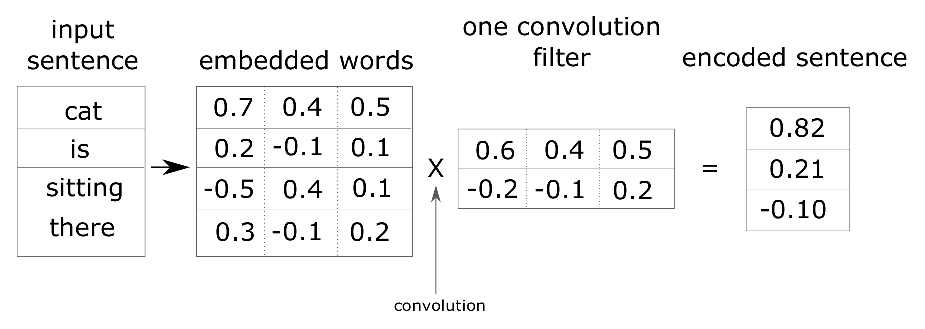
\includegraphics[width=13cm]{1d_conv.eps}
	\centering
	\caption{Sentence encoding using a 1D convolution with one filter.}
	\label{1d_conv}
\end{figure} 

\paragraph{}
Last but not least, there is a possibility to use pre-trained models such as BERT or GPT-2. These are powerful models trained for a couple of days on large clusters and are usually only fine-tuned during training on a final task. In other words, it is not feasible to train them on a custom dictionary from scratch in this work. That is a major drawback for the Stackoverflow dataset due to the specific dictionary of the users. Moreover, the posts contain code snippets for which neither the BERT nor GPT-2 is pre-trained.

\subsection{Word Embedding}\label{word_embedding_analysis}
\paragraph{}
A lot of neural network models dealing with similar problems use pre-trained word embeddings. The reason is either to save a training time or to cope with a lack of labeled data. This work also chooses to utilize pre-trained embeddings for both textual parts of the posts and parts containing code. The reason is mainly to speed up the training.

\paragraph{}
The major questions regarding word representations are which embedding technique to use and how to treat the code. One approach that can be seen in work from Facebook \cite{facebook0_unsupervised} is to use a Fasttext (a variant of the Word2Vec) and to remove all special characters and programming language reserved tokens from the code. The result is a sequence made up of identifiers only.

\paragraph{}
This approach does not seem to be beneficial for this work since the mentioned preprocessing of the code results in losing information about the programming language. Moreover, it relies on using identifiers with reasonable names. For this work, it is essential  to preserve the information about the used programming language, since this may be the major difference between the two questions. Similarly, the proposed models shall not rely on the usage of meaningful identifiers. This is because the questions may refer to a general feature of the programming language and the code snippet might not be supposed to do a meaningful activity.

\paragraph{}
These facts lead to choosing a different approach for code embedding, where the reserved words and special characters are processed by the network as well. Therefore, the $k$ most common tokens in the complete dictionary (including tokens such as "\{", "\}" or "public") are used to pre-train their embeddings and the rest of them is handled as OOVs. It can be assumed that all the OOVs that appear in the code are variable or function identifiers.

\paragraph{}
Another important decision is the way how to treat OOVs. To handle them, this work creates a special "<OOV>" token, whose representation is learned during the end to end training, while the rest of the embeddings are pre-trained and fixed. Additionally, representations of other special tokens described in section \ref{preprocessing} are pre-trained as well. Other possible ways of how to handle the OOVs are subword models (section \ref{subword_models}), character level embedding, or a mixture of the word and character level embedding.

\paragraph{}
To pre-train the embeddings, this work chooses to work with the Word2Vec - CBOW model, which is a frequent choice of many related works. Moreover, there is a pre-trained Word2Vec model available on a Tensorflow Hub, which can be used for a comparison with the custom trained embeddings.

%Why pre-training? \\ 
%GloVe, Word2Vec, Fasttext, subword models -> why W2V was chosen??? \\
%how to handle OOVs?

\section{Architecture}
\paragraph{}
Generally, the proposed models use siamese neural network architecture (section \ref{siamese_nn}), which is illustrated in figure \ref{siamese_nn}. The siamese neural network in the picture accepts two questions, applies pre-trained embeddings and passes them through subsequent layers that share their weights between both branches. That results in generating a vector representation of both questions. These vectors are merged and passed through a multi-layer perceptron with a softmax layer at the end.

\begin{figure}[!h]
	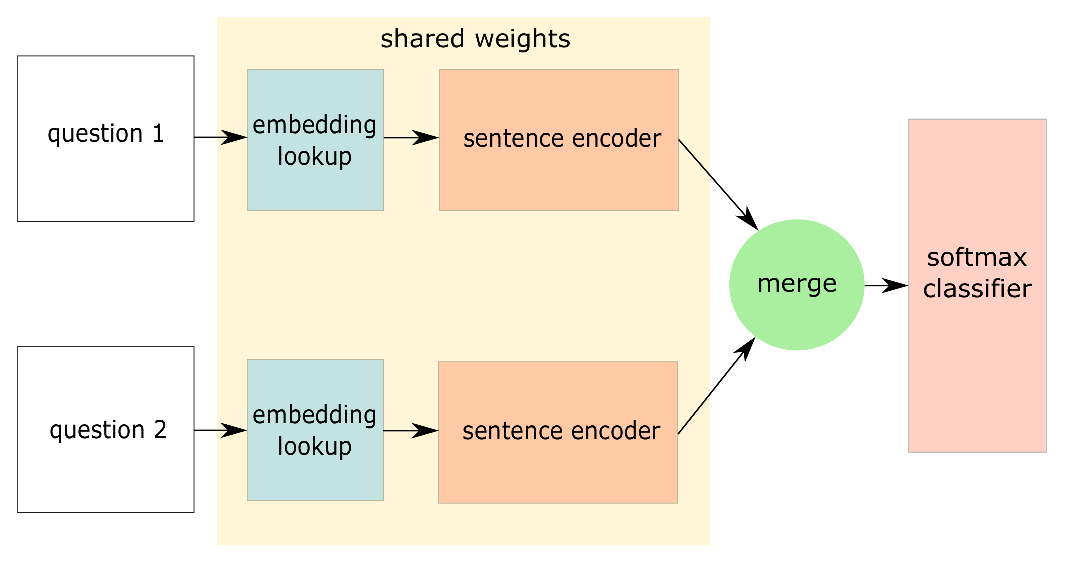
\includegraphics[width=13cm]{siamese_nn.eps}
	\centering
	\caption{Siamese neural network architecture for classification on the Stackoverflow dataset.}
	\label{siamese_nn}
\end{figure}

\paragraph{}
The most remarkable difference between proposed models is a sentence encoder, while the general architecture is the same. Other minor differences can be found in a softmax classifier part as well. These can be, for example, a number of layers or a number of neurons in the layers.

\paragraph{}
The subsequent sections firstly introduce common features of all the models and then the individual models are described in detail.

\subsection{Common Features}
\paragraph{}
All the proposed models share common architectural elements such as an input pipeline, embedding layer, the way how sentence vectors are merged, metrics and loss. These common features are discussed in this section.

\subsubsection{Data input}
\paragraph{}
The question pairs are fed into the model in batches of a parametrizable size. An input pipeline takes care of loading the data, padding the sentences to the same length, shuffling and batching. The yielded batch contains pairs of sequences created from dictionary indexes of each word. Put differently, the input is a tensor of shape \textit{(2, batch size, max sequence length)}.

\subsubsection{Embedding Lookup}
\paragraph{}
The first layer of each model is an embedding layer (\textit{tf.keras.layers.Embedding}), whose weight matrix is initialized with the pre-trained embedding weights. The embedding layer creates a matrix made up of one-hot vectors that correspond to the dictionary indexes of fed-in words. The matrix is then multiplied with the weight matrix, which results in a tensor with shape (\textit{batch size, max sequence length, embedding dimension}) for each of the input questions. A way how the OOVs are handled is similar for all the models and is described in section \ref{word_embedding_analysis}.

\subsubsection{Merge Step}
\paragraph{}
Another common feature of all the models is the merging of sentence representations. All proposed models work with a concatenation of the sentence vectors, which is also used in the SNLI dataset paper \cite{snli}.

\subsubsection{Optimized Metric}
\paragraph{}
The choice of a metric (section \ref{metrics}) to be optimized and observed is very important. This work aims to optimize an f1 score since table \ref{dataset_final_counts} shows that the dataset is unbalanced. It means that accuracy would not provide interpretable results. Besides, a confusion matrix is used to provide more in-depth insight into the model’s behavior.

\subsubsection{Loss Function}
\paragraph{}
An originally used loss function was a cross-entropy (section \ref{cross_entropy}), which is a frequent choice of classification tasks with a softmax output layer. However, experiments showed that the cross-entropy does not correlate with the f1 score very well, causing worse results. To address this problem, an f1 loss (section \ref{f1_loss}) is used for training the models and is optimized using an Adam optimizer (section \ref{optimizers}). 

\subsubsection{Regularization}
\paragraph{}
A regularization (section \ref{other_nn_architectrues_and_techniques}) is an integral part of a neural network. The models proposed in this work use an L2 regularization (\textit{tf.keras.regularizers.l2}) in all the layers of the softmax classifier. A regularization parameter is always the same for all the layers.

\paragraph{}
Additionally, the models utilize dropout layers (\textit{tf.keras.layers.Dropout}). In the models, two different dropout configurations are used. The first one (which is usually configured to a higher dropout rate) is always after the embedding layer. The second dropout follows each of the subsequent layers.

\subsection{Word Summation}
\paragraph{}
The first proposed model (figure \ref{word_summation_model_figure}) is based on a word summation method described in section \ref{word_averaging}. It means that the whole sentence encoder is just a sum of the word embeddings. Encoded questions are then concatenated and passed through a dense layer and a softmax layer at the output. This model uses only a textual part of the dataset while omitting code tokens entirely  (except the special "<code>" replacement token in the text).

\paragraph{}
This model is used in two variants that differ in a number of classes. A two-class model is a special case of a three-class model, where all the "similar" samples are treated as "different".


\begin{table}[!h]
	\begin{center}
		\begin{tabular}{l c} 
			\hline
			\textbf{Variant} & \textbf{Classes} \\ [0.5ex] 
			\hline\hline
			WordSum2Cls & 2 \\ 
			WordSum3Cls & 3\\ 
			\hline
		\end{tabular}
	\end{center}
	\caption{Variants of a word summation model.}
	\label{word_summation_variants}
\end{table}

\begin{figure}[!h]
	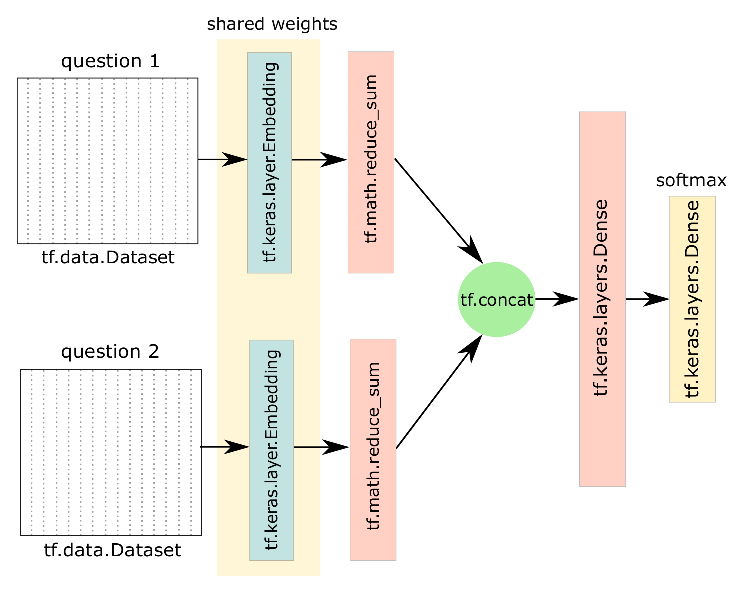
\includegraphics[width=13cm]{word_summation.eps}
	\centering
	\caption{Neural network model based on a word embedding summation. Dropout layers are omitted in the picture for the sake of readability.}
	\label{word_summation_model_figure}
\end{figure}


\subsection{BiLSTM Encoder}
\paragraph{}
The second proposed model is based on a bidirectional LSTM encoder and utilizes only the textual part of the dataset. Figure \ref{bi_lstm_encoder} shows one variant of the model, where the embedded sequences are passed through two BiLSTM layers that produce the vector representation of the sentences. The resulting representations are concatenated and used for classification in the softmax classifier.

\paragraph{}
Variants of the model differ in a number of classes, a number of BiLSTM layers in the encoder and a number of the dense layers in the softmax classifier. These variants are described in table \ref{bi_lstm_encoder_variants}.

\begin{figure}[!h]
	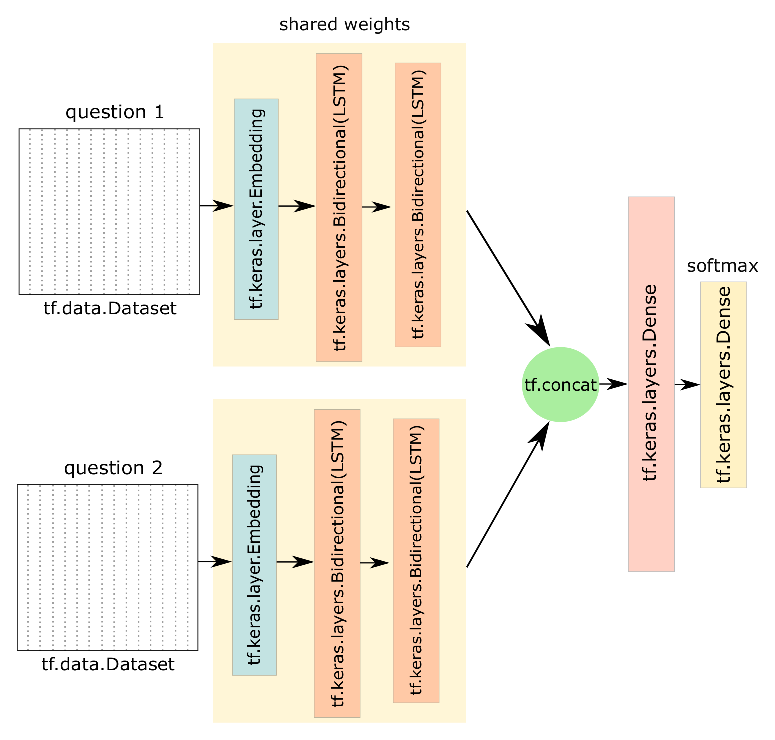
\includegraphics[width=14cm]{bi_lstm_encoder.eps}
	\centering
	\caption{A bidirectional LSTM encoder model. Dropout layers are omitted in the picture for the sake of readability.}
	\label{bi_lstm_encoder}
\end{figure}

\begin{table}[!h]
	\begin{center}
		\begin{tabular}{l c c c } 
			\hline
			\textbf{Variant} & \textbf{Classes} & \textbf{BiLSTM} & \textbf{Dense} \\ [0.5ex] 
			\hline\hline
			BiDirLSTM1L3Cls & 3 & 1 & 1 \\ 
			BiDirLSTM2L3Cls & 3 & 2 & 1 \\ 
			BiDirLSTM1L2Cls & 2 & 1 & 1 \\ 
			BiDirLSTM2L2Cls & 2 & 2 & 1 \\ 
			BiDirLSTM2LDense2L2Cls & 2 & 2 & 2 \\ 
			BiDirLSTM2LDense2L3Cls & 3 & 2 & 2 \\ 
			\hline
		\end{tabular}
	\end{center}
	\caption{Variants of a BiLSTM encoder model.}
	\label{bi_lstm_encoder_variants}
\end{table}

\subsection{BiLSTM Code Encoder}
\paragraph{}
The last proposed model (figure \ref{bi_lstm_code_encoder}) is different from the previous one in a way how the code parts of the dataset are handled since this model also utilizes the second part (with code tokens) of the dataset. It means that the model accepts four sequences - two of them carry the textual tokens and the others carry the code tokens. The textual sequences are then embedded using the pre-trained embeddings for text, whereas the code sequences are embedded using embeddings trained for code.

\paragraph{}
The sentence encoder is separated into two parts - an encoder for code and an encoder for text. The structure of both of them is identical since they are made up of two bidirectional LSTM layers. However, the encoders do not share their weights completely. The way how the weights are shared is marked out by yellow and blue background in the figure.

\paragraph{}
A result of passing the question through the embedding layer and the encoder is a vector representation of the code contained in the question as well as a representation of the text. These two representations are concatenated, and together they form a complete representation of the entire question. The fact that this model utilizes the complete information from the question is a significant  advantage of this model. Thanks to that, the model can provide better results since it can distinguish, for example, the programming language of the code snippets. 

\paragraph{}
To illustrate how the code processing can help to improve the accuracy of the model, imagine two questions where users ask "How to implement synchronization of threads t1 and t2 into the following code". For a model that only has the text of the questions, not the code snippet, these questions appear the same. However, if the code of the first query is written in Java and the second in C, the two questions are clearly different.

\paragraph{}
Finally, the representations of the questions are concatenated and processed by a softmax classifier with two dense layers and a softmax layer on the top. The code encoder model is trained in a variant with two and three classes (table \ref{bi_lstm_code_encoder_variants}).

\begin{table}[!h]
	\begin{center}
		\begin{tabular}{l c} 
			\hline
			\textbf{Variant} & \textbf{Classes}\\ [0.5ex] 
			\hline\hline
			BiDirCodeEncoder2L2Cls & 2 \\ 
			BiDirCodeEncoder2L3Cls & 3 \\ 
			\hline
		\end{tabular}
	\end{center}
	\caption{Variants of a BiLSTM encoder model.}
	\label{bi_lstm_code_encoder_variants}
\end{table}

\begin{figure}[!h]
	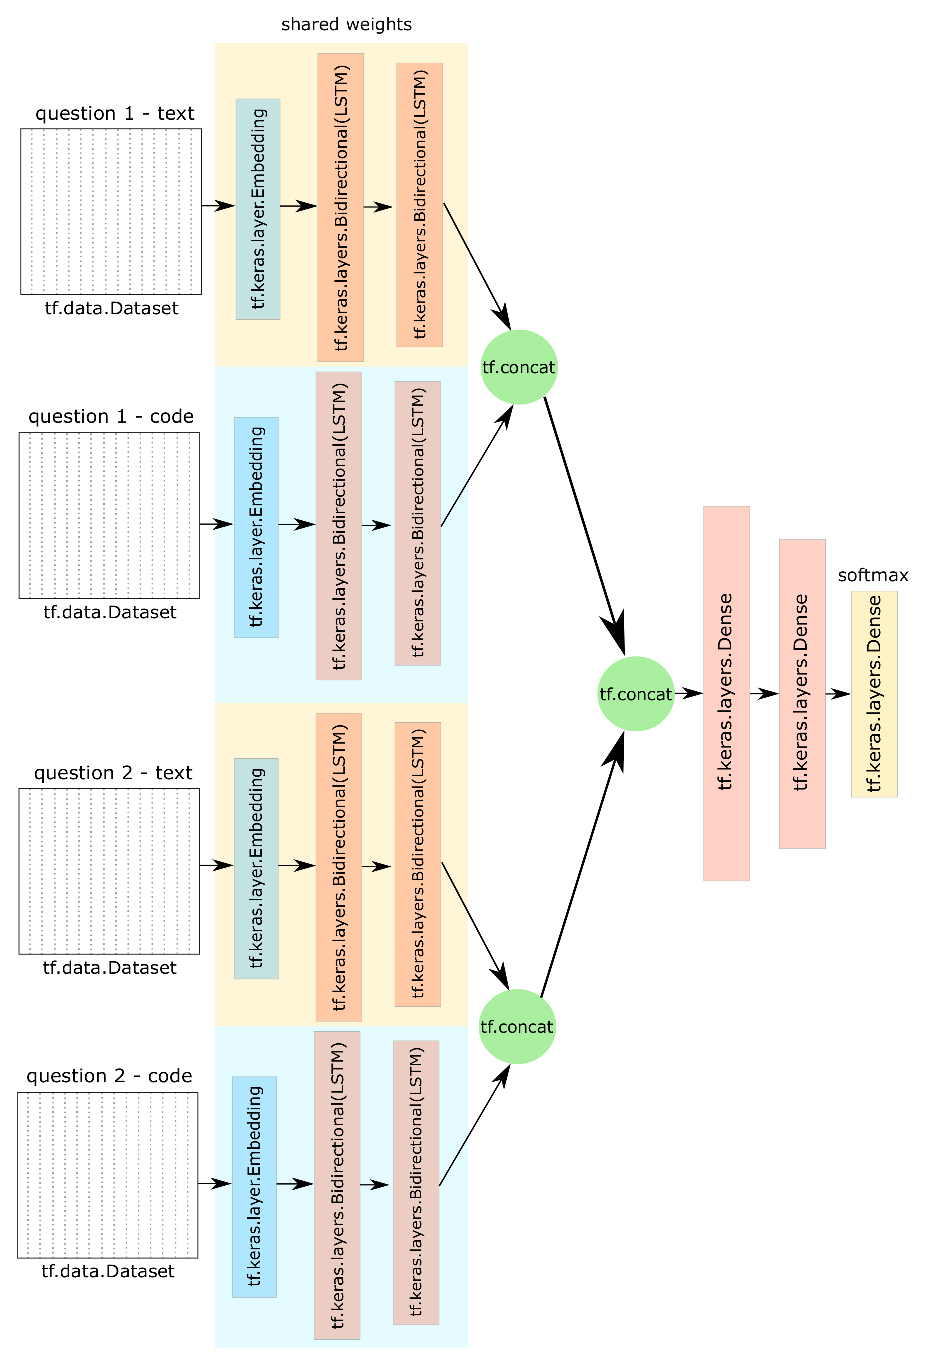
\includegraphics[width=14cm]{bi_lstm_code_encoder.eps}
	\centering
	\caption{A bidirectional LSTM code encoder model. Dropout layers are omitted in the picture for the sake of readability.}
	\label{bi_lstm_code_encoder}
\end{figure}



%Maily to describe my architectures in detail. Other approaches described in previous section.
%siamese NN \\
%baseline model -> summarizing and averaging\\
%BiLSTM \\ 
%BiLSTM with code \\




\chapter{Results and Evaluation}\label{results}
\paragraph{}
This chapter aims to discuss the results achieved using the models proposed in chapter \ref{analysis}. Furthermore, the chapter provides a more detailed description of realizing the chosen approaches. The first section discusses a data pipeline, while in the second section, the setup of hyperparameters is stated. Since numerous experiments are done for each of the model variants using different hyperparameters, only the configuration leading to the best result of the given model is stated. After that, the second section states the achieved results and compares them with existing work on the SNLI (section \ref{snli}) dataset. Finally, the results are further analyzed to provide deeper insights into the accuracy.

\section{Data Pipeline Construction}
\paragraph{}
This section describes the steps taken to prepare data for the neural network. In the first part, details of indexing the Stackoverflow data into Elasticsearch are discussed. In contrast, the second part describes how the data are exported from the Elasticsearch into a form usable by input pipelines.

\subsection{Indexing Data into Elasticsearch}\label{indexind_the_data}
\paragraph{}
As stated in section \ref{assembling_the_dataset}, it is necessary to store the data in the Elasticsearch to assemble the dataset. Therefore, an Elasticsearch cluster made up of three nodes is established. The cluster is running on virtual machines provided by the MetaCentrum (\url{https://metavo.metacentrum.cz}). The machine running the cluster's master node also hosts a Kibana instance to facilitate exploration of the data in the cluster.

\paragraph{}
To index the data, a Logstash utility is used. Using the Logstash, one can configure an input pipeline that processes a given stream of data and ingest them into a configured Elasticsearch instance. The Logstash input pipelines used for this work consist of three primary operations - input, filter and output. The input operation ingests the given XML file into the pipeline. Then the filter operation takes care of parsing the XML and selecting desired fields. Finally, the output operation of the pipeline assembles a document and sends it to the Elasticsearch instance.

\subsection{Dataset Export}
\paragraph{}
According to a description in section \ref{assembling_the_dataset}, the dataset is assembled and resulting assignments of the posts are stored in the Elasticsearch database. The assignments are represented by dataset groups and post roles. In each group there is a \textit{master post} and a number of \textit{duplicate}, \textit{similar} and \textit{different} posts. Based on that, the dataset export is created.

\paragraph{}
The process of dataset export iterates over all the \textit{master posts} and queries all remaining posts in the corresponding dataset group. Each of these posts is then used in a pair with the \textit{master post} and together, they represent one example. The corresponding class is derived from the role of the post, not being the \textit{master}.

\paragraph{}
The individual dataset examples are exported into a CSV file with format: "\textit{first\_post\_ID};\textit{second\_post\_ID};\textit{class}". Furthermore, to be able to use a faster variant of the proposed input pipeline (section \ref{input_pipelines}), two additional CSV files are created. One of them contains the corresponding preprocessed text of the posts and the second one consists of preprocessed code. The resulting dataset is split into three distinct parts, as shown in table \ref{dataset_final_counts}.

\begin{table}[h!]
	\begin{center}
		\begin{tabular}{l || r r r r} 
			\hline
			\textbf{Type} & \textbf{Train} & \textbf{Dev} & \textbf{Test} & \textbf{Total} \\ [0.5ex] 
			\hline\hline
			Different & 550 757 & 64 615 & 32 448 & 647 820 \\
			Similar & 526 759 & 62 010 & 30 790 & 619 559 \\
			Duplicates & 191 931 & 22 721 & 11 437 & 226 089 \\
			\hline
			Total & 1 269 447 & 149 346 & 74 675 & 1 493 468 \\
			\hline
		\end{tabular}
	\end{center}
	\caption{Stackoverflow dataset example count summary.}
	\label{dataset_final_counts}
\end{table}

\section{Experimental Setup}
%Hyperparameters and model setup
%Which techniques and settings improved the results and which one did not
\paragraph{}
In the previous chapter, the architecture of the models is discussed. However, the setup of hyperparameters and other essential settings are not mentioned there at all. Therefore, this section discusses the hyperparameter setup using which the best results are achieved.

\subsection{Embedding}
\paragraph{}
As stated in chapter \ref{analysis}, the work utilizes pre-trained Word2Vec embeddings for both code and textual parts. These embeddings are joint for all the models and are trained on a whole set of posts from the Stackoverflow (chapter \ref{dataset}). Since experiments show that fine-tuning the embeddings during an end to end training does not improve the results at all, the pre-trained embeddings are fixed and are not fine-tuned during the training.

\paragraph{}
The embeddings are pre-trained using a CBOW variant of a Word2Vec (section \ref{w2v}) with negative sampling. The window size for training is set to five words. A dictionary for the textual embeddings is composed of all words that appear in a corpus at least 50 times. For the embeddings of the code parts, the minimum occurrence threshold is set to 500 occurrences.

%CBOW, window=5, negative sampling
%min frequency code - 500x
%              text - 50x

\subsection{Word Summation Model}
\paragraph{}
The word summation model turns out to show the best results while using the two-class variant (\textit{WordSum2Cls}) in combination with an f1 loss. Experimentally set hyperparameters are:

\begin{itemize}
	\item batch size: 256
	\item length of input sequences: 150
	\item number of neurons in the first dense layer: 128
	\item the activation function in the first dense layer: ReLu
	\item L2 regularization factor in the dense and softmax layer: 0.05
	\item first dropout rate (after embedding): $0.5$
	\item second dropout rate (all the others): $0.35$
\end{itemize}

\subsection{BiLSTM Encoder}
\paragraph{}
%BiDirLSTM2LDense2LConcat2Cls, f1 loss
% 1. droput: 0.5, 2. dropout: 0.35, batch size:256, seq_len:150, l2 reg: 0.05
% first BiLSTM layer: 256
% second BiLSTM layer: 128
% first Dense layer: 128
% second Dense layer: 64
The most successful BiLSTM encoder model is the two-class variant with two LSTM layers in the encoder and two dense layers preceding the softmax layer (\textit{BiDirLSTM2LDense2L2Cls}). A used loss function is an f1 loss. Experimentally set hyperparameters are:

\begin{itemize}
	\item batch size: 256
	\item length of input sequences: 150
	\item size of the first BiLSTM layer: 256
	\item size of the second BiLSTM layer: 128
	\item number of neurons in the first dense layer: 128
	\item number of neurons in the second dense layer: 64
	\item the activation function in the first two dense layers: ReLu
	\item L2 regularization factor in the dense and softmax layers: 0.05
	\item first dropout rate (after embedding): $0.5$
	\item second dropout rate (all the others): $0.35$
\end{itemize}

\subsection{BiLSTM Code Encoder Model}
\paragraph{}
% 2 class, f1 loss
% batch size: 256
% first dropout: 0.45, second dropout: 0.3
% sequence length: 250
% first BiLSTM layers: 256
% second BiLSTM layers: 128
% first dense layer: 256
% second dense layer: 128
The last model that uses a code encoder alongside the textual encoder shows the best results in the two-class variant with an f1 loss. The values of the hyperparameters are the same for both encoders and are therefore stated only once in a listing. The used hyperparameter values are:

\begin{itemize}
	\item batch size: 256
	\item length of input sequences: 250
	\item size of the first BiLSTM layers: 256
	\item size of the second BiLSTM layers: 128
	\item number of neurons in the first dense layer: 256
	\item number of neurons in the second dense layer: 128
	\item the activation function in the first two dense layers: ReLu
	\item L2 regularization factor in the dense and softmax layers: 0.05
	\item first dropout rate (after embedding): 0.45
	\item second dropout rate (all the others): 0.3
\end{itemize}

\paragraph{}
Before presenting results achieved using these hyperparameters, it should be pointed out, that the dropout rates are configured to high values for all the models. Decreasing the rates results in significantly lower f1 scores. Additionally, it is important to disable a bias in the softmax output layer to prevent the models from learning a strong bias towards more numerous classes.  

\section{Model Results Evaluation}
\paragraph{}
%compare performance of baseline model and BiLSTM model resutlts to corresponding results on SNLI
%which techniques improved the results and which one did not
Tables \ref{2class_results} and \ref{3class_results} state achieved results of the proposed models on the Stackoverflow dataset. The tables are separate for two-class and three-class models since the results are not easily comparable, as discussed later.

\begin{table}[!h]
	\centering
	\begin{tabular}{l:lr:lr:lr} 
		\hline
		\multicolumn{1}{c:}{\multirow{2}{*}{ \textbf{Model} }} & \multicolumn{2}{c:}{\textbf{Train} } & \multicolumn{2}{c:}{\textbf{Dev} } & \multicolumn{2}{c}{\textbf{Test} }  \\
		\multicolumn{1}{c:}{}& Acc & F1 & Acc & F1 & Acc & F1 \\ 
		\hline\hline
		BiDirCodeEncoder2L2Cls & 88.0 & 75.8 & 86.9 & 74.6 & 86.1 & 74.1 \\
		BiDirLSTM2L2Cls & 84.2 & 70.8 & 84.0 & 70.6 & 83.9 & 71.0 \\
		BiDirLSTM2LDense2L2Cls & 84.0 & 70.8 & 85.5 & 70.7 & 84.6 & 70.9 \\
		BiDirLSTM1L2Cls & 84.1 & 70.4 & 85.0 & 70.5 & 84.7 & 70.8 \\
		WordSum2Cls & 84.3 & 70.1 & 84.5 & 69.2 & 86.2 & 68.8 \\
		\hline
	\end{tabular}
	\caption{Results of two-class models.}
	\label{2class_results}
\end{table}

\begin{table}[!h]
	\centering
	\begin{tabular}{l:lr:lr:lr} 
		\hline
		\multicolumn{1}{c:}{\multirow{2}{*}{ \textbf{Model} }} & \multicolumn{2}{c:}{\textbf{Train} } & \multicolumn{2}{c:}{\textbf{Dev} } & \multicolumn{2}{c}{\textbf{Test} }  \\
		\multicolumn{1}{c:}{}& Acc & F1 & Acc & F1 & Acc & F1 \\ 
		\hline\hline
		BiDirCodeEncoder2L3Cls & 88.2 & 81.6 & 86.6 & 80.2 & 85.3 & 79.2 \\
		BiDirLSTM2LDense2L3Cls & 86.0 & 78.0 & 86.6 & 78.0 & 85.9 & 78.1 \\
		BiDirLSTM2L3Cls & 85.6 & 77.6 & 87.4 & 76.8 & 87.2 & 77.5 \\
		BiDirLSTM1L3Cls & 85.5 & 77.6 & 86.4 & 77.1 & 85.8 & 77.5 \\
		WordSum3Cls & 84.6 & 76.8 & 85.1 & 77.0 & 86.7 & 75.1 \\
		\hline
	\end{tabular}
	\caption{Results of three-class models.}
	\label{3class_results}
\end{table}

\paragraph{}
The results show that the most successful models were the BiLSTM code encoders. That confirms the assumption that discarding the code contained in most queries can lead to a significant loss of information. Moreover, the word summation model was the least successful one, which was, however, expected since it is a baseline model. The difference in a test f1 score between the baseline models and BiLSTM code encoders is $5.3\%$ and $4.1\%$ for the two-class and three-class models respectively.

\paragraph{}
An interesting observation that can be done on the results is that the architecture variant of BiLSTM encoder does not play an important role in the resulting f1 score. In other words, it can be seen that neither an expansion of the softmax classifier part nor an expansion of the encoder improved the f1 score in a significant way.

\paragraph{}
Furthermore, it can be noticed that the three-class models report much better results than the two-class models. As a matter of fact, this observation might be misleading since a more in-depth analysis of confusion matrices shows that the two-class models work slightly better. That can be seen in figures \ref{bi_lstm_code_encoder_2cls_conf_mat} and \ref{bi_lstm_code_encoder_3cls_conf_mat}. The figures show that despite the higher f1 score, the three-class models classify fewer duplicates correctly than the two-class models do. Even though this phenomenon is demonstrated on the BiLSTM code encoder, it applies to all the proposed models in the same way.

\begin{figure}[!h]
	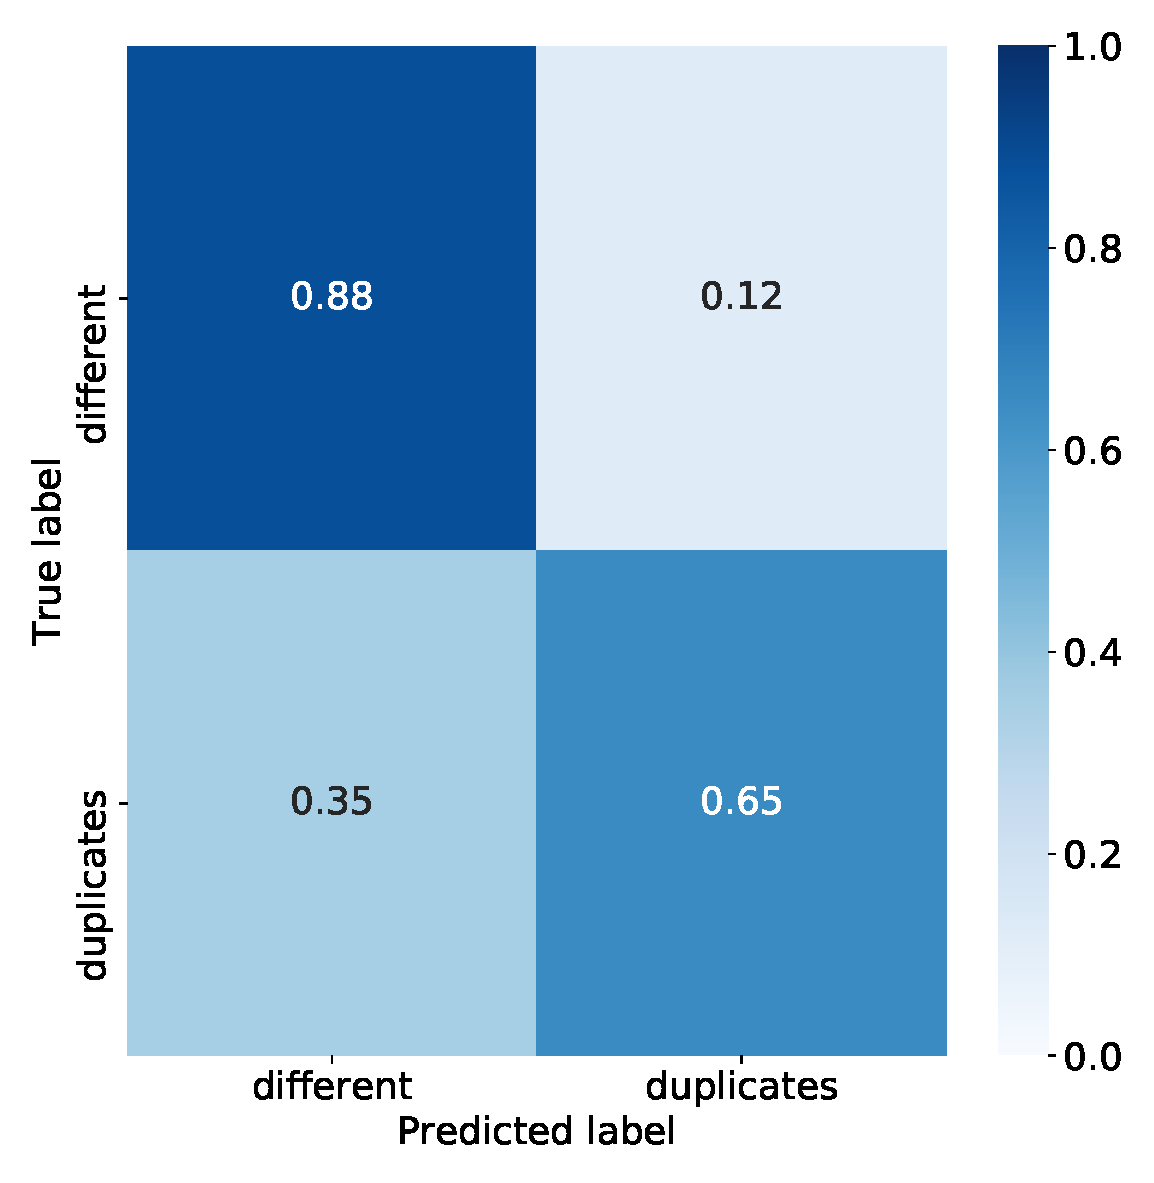
\includegraphics[width=8cm]{BiLSTMCodeEncoder2Cls_conf_mat.eps}
	\centering
	\caption{A confusion matrix for the two-class variant of the BiLSTM code encoder model on a test dataset split.}
	\label{bi_lstm_code_encoder_2cls_conf_mat}
\end{figure}

\begin{figure}[!h]
	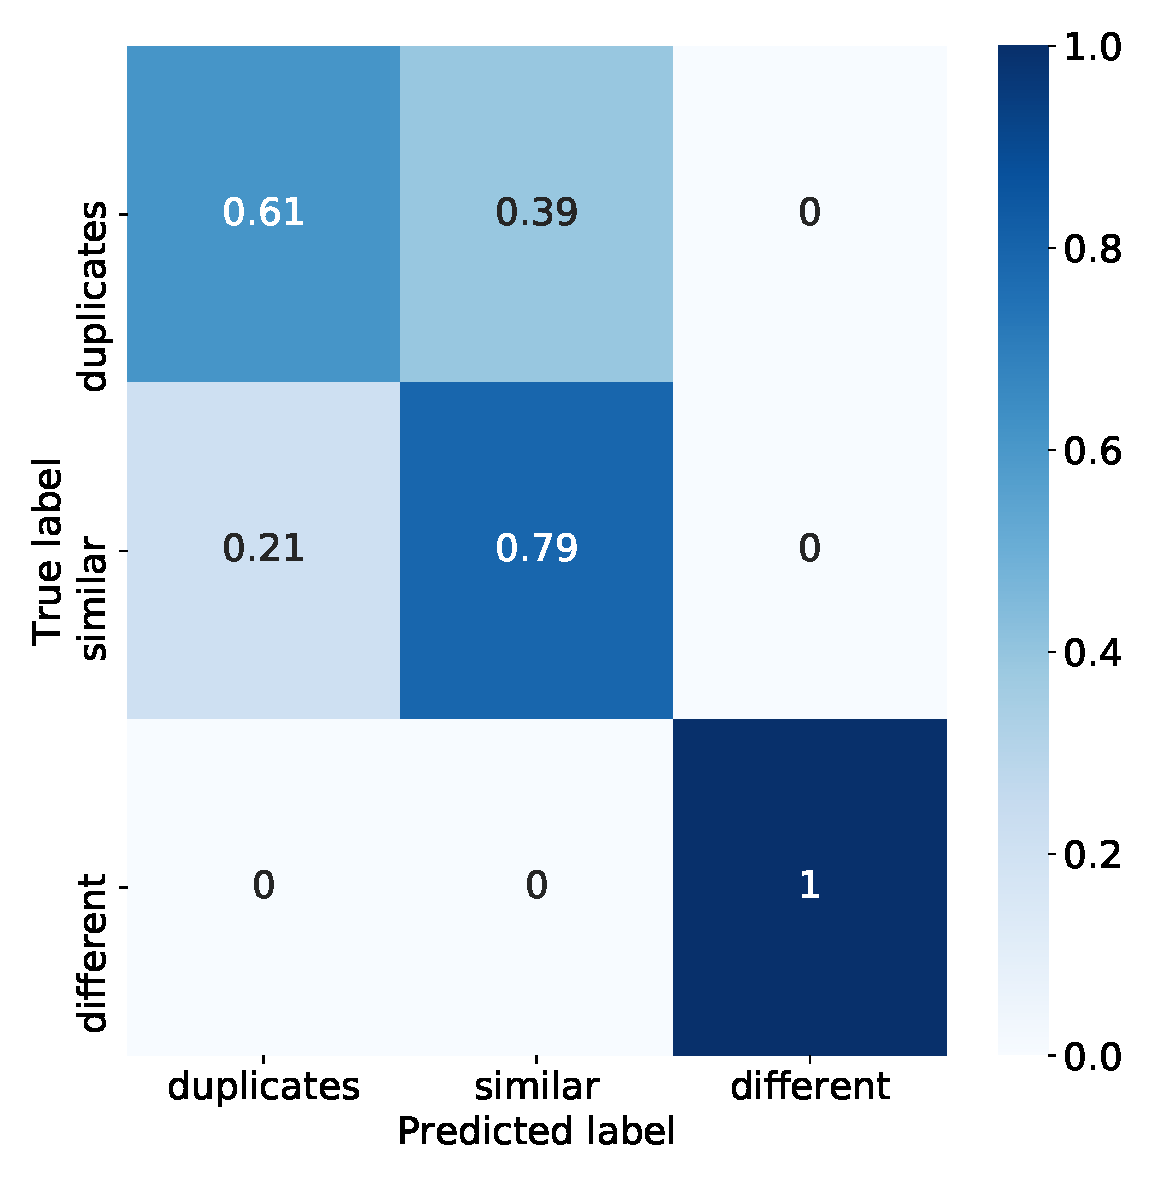
\includegraphics[width=8cm]{BiLSTMCodeEncoder3Cls_conf_mat.eps}
	\centering
	\caption{A confusion matrix for the three-class variant of the BiLSTM code encoder model on a test dataset split.}
	\label{bi_lstm_code_encoder_3cls_conf_mat}
\end{figure}

\subsection{Other experiments}
\paragraph{}
Developing and fine-tuning the model requires a lot of experiments and testing of various techniques. In this work, these are mainly a different loss function and a different merging step. This section briefly discussed the results and conclusions of these experiments.

\paragraph{}
An originally used loss function was a cross-entropy, which correlates very well with accuracy. Unfortunately, with the cross-entropy loss function, the models tend to learn a strong bias towards more numerous classes such as \textit{similar} or \textit{different}, not classifying the \textit{duplicate} examples correctly. To address this problem, the f1 loss function is used instead and it brings a significant improvement observed in both the f1 score and confusion matrix. The improvement of the f1 score achieved by using the f1 loss is around $2\%$ on average.

\paragraph{}
Additionally, the work also investigated the possibility of using the absolute value of an element-wise subtraction as a way of merging the sentence representations. However, this merging technique turns out not to be working very well. As a matter of fact, the absolute difference worsens the f1 score by about $4\%$.

\subsection{Comparison to SNLI}
\paragraph{}
Classification on the SNLI dataset is, to some extent, similar to the task of recognizing duplicate questions. At least the proposed three-class architectures, except the BiLSTM code encoders, apply to this task, which is why the SNLI dataset has been used to verify the proposed models.

\paragraph{}
Since the SNLI dataset does not contain any code, the only models used for the verification on the SNLI are the word summation and BiLSTM encoder models. The results of these models (table \ref{models_vs_snli}) without any architectural change are significantly lower than those presented in \cite{snli} with similar models. However, this is expected since the models proposed in this work are tailored and fine-tuned to a slightly different task and the main aim of this work is to optimize the results for the Stackoverflow dataset, not for the SNLI.

\begin{table}
	\centering
	\begin{tabular}{lr} 
		\hline
		\textbf{Model}          & \multicolumn{1}{l}{\textbf{Test accuracy}}  \\ 
		\hline\hline
		LSTM RNN \cite{snli}    & 77.6                              \\
		Sum of words \cite{snli}& 75.3                              \\
		BiDirLSTM2L3Cls        & 72.1                               \\
		WordSum3Cls            & 69.7                               \\
		\hline
	\end{tabular}
	\caption{An accuracy comparison of the proposed models with the work \cite{snli} on the SNLI dataset.}
	\label{models_vs_snli}
\end{table}


\section{Manual Analysis of Dataset and Errors}\label{analysis_of_dataset_and_errors}
\paragraph{}
The previous section of this chapter states the results we achieved using the proposed models. However, the measured metrics,  such as the f1 score and confusion matrix, heavily depend on having the dataset labeled precisely. In our case, the dataset is extracted from a public webpage with millions of users, and therefore, it can be expected that the dataset may be subject to many errors. More precisely, we assume that some amount of duplicate links may be erroneous. Therefore, we create a manual survey of a subset of question pairs, which shall provide us more profound insights into the achieved results.

\paragraph{}
The subset of question pairs to be analyzed is made up of 100 samples. The first 50 of them are randomly sampled from the dataset examples labeled as \textit{duplicate}. Next 25 samples are chosen from duplicate pairs that are erroneously classified as \textit{different} (type I error) by our \textit{BiLSTM Code Encoder} model. Finally, the remaining 25 samples are chosen from non-duplicate pairs of questions, erroneously classified as \textit{duplicate} (type II error).

\paragraph{}
For each of the survey samples, we asked three independent people who work or study in the information technologies field, to asses whether the questions are duplicates or not. To determine the resulting class for each of the pairs, we choose the predominant answer (answer with two or three votes).

\paragraph{}
The results of the survey are summarized in table \ref{manual_surver_results}. The manual analysis shows that the dataset comprises a not negligible amount of redundant duplicate links. This can heavily affect the results obtained by the neural network and therefore, this shall be considered when evaluating the results. For a detailed listing of respondent answers, see appendix \ref{manual_analysis}.

\smallskip{}
\begin{table}[!h]
	\centering
	\begin{tabular}{l c c c} 
		\hline
		\textbf{Survey subset} & \textbf{Samples total} & \textbf{Duplicates \#} & \textbf{Duplicate \%}  \\ 
		\hline\hline
		random duplicates & 50 & 36 & 72\% \\
		type I error      & 25 & 13 & 52\% \\
		type II error     & 25 & 3  & 12\% \\
		\hline
	\end{tabular}
	\caption{Results of manual survey of the dataset samples. The samples are divided into three categories based on the how they are chosen for the survey.}
	\label{manual_surver_results}
\end{table}


\section{Results Discussion}
\paragraph{}
%- why the f1-score is not too high\\
%- a tendency to mar non-duplicates as duplicates \\
%- some queried similar questions can be duplicated \\
%- a lot of duplicates may not be marked as a duplicate\\
This section builds on the results presented in the previous sections, discussing in more detail why the models can detect at most 65\% of the duplicates. The discussion is mainly from the source data point of view since it can play a significant role in the achieved f1 score. 

%- a tendency to mark non-duplicates as duplicates
\paragraph{}
A first phenomenon that can be observed on the Stackoverflow website is that users often mark questions as duplicates, although the questions focus on slightly different topics. Therefore, the data source contains a not negligible amount of false-positive examples, which have a negative consequence on the network's metrics. We substantiate this statement by manual analysis of the dataset samples (section \ref{analysis_of_dataset_and_errors}), which shows that the proportion of false-positive samples in the dataset is around one quarter.

\paragraph{}
Furthermore, the manual analysis shows that among the dataset examples labeled as \textit{duplicate} but classified as \textit{different} is roughly 48\% of false-positives. If we consider this fact, we get 81\% precision on the duplicate questions, which is a significant improvement over the measured 65\%.

\paragraph{}
Unlike the false-positives, the false-negative examples are not so abundant among the \textit{different} pairs classified as \textit{duplicate} since they make up only 12\% of the errors. Taking this into consideration, we get 89\% precision on the non-duplicate questions. A cause of the false-negative examples is the dataset assembly algorithm (section \ref{assembling_the_dataset}). It is because the dataset shall contain semi-positive samples that are collected by Elasticsearch's full-text queries, which may find unmarked duplicated questions.

\paragraph{}
Based on the manual analysis of errors, we create an estimation of a confusion matrix showing the network results not being affected by errors in the evaluation data. The resulting confusion matrix is depicted in figure \ref{bi_lstm_code_encoder_2cls_conf_mat_correction}. However, it shall be further noted that the accuracy of the network might increase if being trained on data free from such errors.


\paragraph{}
\begin{figure}[!h]
	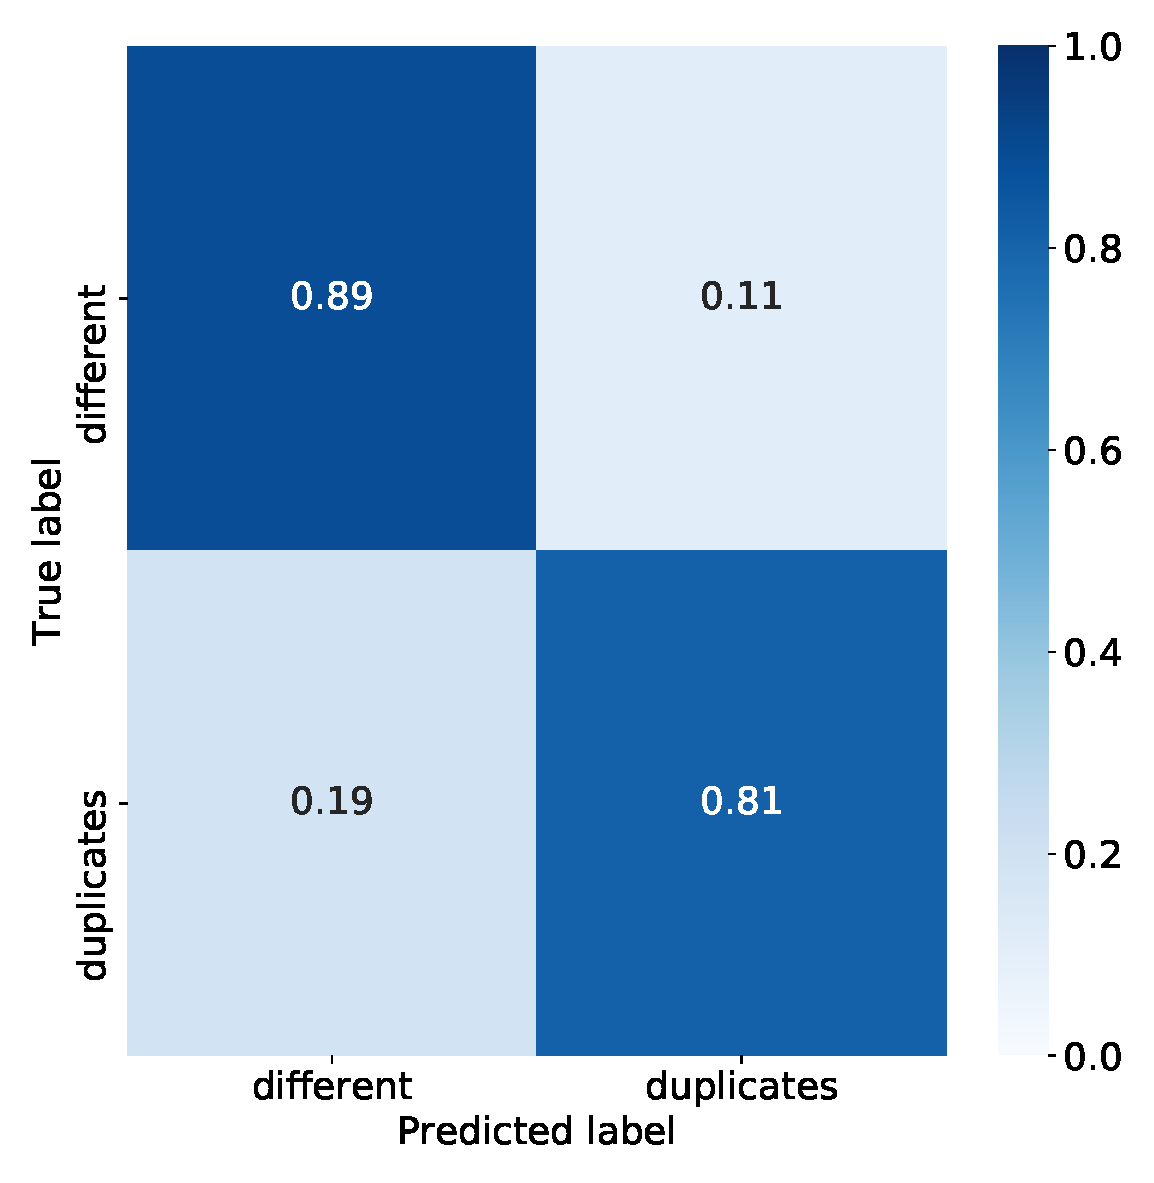
\includegraphics[width=8cm]{BiLSTMCodeEncoder2Cls_conf_mat_correction.eps}
	\centering
	\caption{Resulting confusion matirx of BiLSTM Code Encoder model after correction based on manual error analysis.}
	\label{bi_lstm_code_encoder_2cls_conf_mat_correction}
\end{figure}


\chapter{Conclusion}
\paragraph{}
In the scope of this work, a new dataset for semantic textual similarity was created from a Stackoverflow data dump. The dataset consists of almost $1.5$ million examples. A learning target of the dataset is to classify whether two questions are duplicates or not. In the future, we are going to release the dataset as an official TF Dataset available for the research community. Furthermore, the work proposed three different siamese neural network architectures to solve this task.

\paragraph{}
The most successful architecture reports a test f1 score of $74.1\%$, improving the f1 score by 5.1\% compared to a baseline model. Furthermore, a manual analysis of duplicate questions and errors suggests that the achieved f1 score is even better. An important feature of our design is a different encoder of code snippets in parallel to a textual encoder. This architectural element enables the network to utilize all the information stored in the data and to make more precise decisions. The proposed models in their hidden layers create a vector representation of sentences that can be obtained and used as a pre-trained sentence embedding for other tasks.

\paragraph{}
This work can be further followed by research into the usage of the obtained sentence representations by integrating them in a Stackoverflow information retrieval or code generation task. For future work, a web application for browsing and searching in the Stackoverflow data was constructed. At the moment, the application provides a standard full-text search only, but it is prepared for integrating with the vector representation based search. Screenshots of the demonstration application can be found in appendix \ref{demo_app}.

\paragraph{}
Moreover, it might be beneficial to explore the usage of self-attention models such as BERT on the created dataset. Even though it would be complicated to train BERT on the code tokens from scratch, it can be used for encoding the textual part alongside the current code encoder. Additionally, the Stackoverflow data contains questions with accepted answers, which could be utilized by another dataset with a learning objective to classify whether a post is an answer to a given question.

\paragraph{}
All source codes used in this work are accessible in a GitHub repository:\\ \url{https://github.com/janpasek97/stackoverflow-siamese-network}.

\chapter*{List of Abbreviations}
\addcontentsline{toc}{chapter}{List of abbreviations}
\begin{itemize}
	\item[] \textbf{API} - application programming interface
	\item[] \textbf{CBOW} - continuous bag of words
	\item[] \textbf{CNN} - convolutional neural network
	\item[] \textbf{DSA} - Dynamic Self-Attention
	\item[] \textbf{FN} - false negative
	\item[] \textbf{FP} - false positive
	\item[] \textbf{GRU} - gated recurrent unit
	\item[] \textbf{LSTM} - long short term memory
	\item[] \textbf{ML} - machine learning
	\item[] \textbf{MSE} - Mean squared error
	\item[] \textbf{NLI} - natural language inference
	\item[] \textbf{NLP} - natural language processing
	\item[] \textbf{OOV} - out of vocabulary
	\item[] \textbf{ReLU} - Rectified linear unit
	\item[] \textbf{RNN} - recurrent neural network
	\item[] \textbf{SNLI} - Stanford Natural Language Inference
	\item[] \textbf{TF} - Tensorflow
	\item[] \textbf{tf-idf} - term frequency - inverse document frequency
	\item[] \textbf{TN} - true negative 
	\item[] \textbf{TP} - true positive 
\end{itemize}
 
% 
% PRO ANGLICKOU SAZBU JE NUTNÉ ZMĚNIT
% CITAČNÍ STYL!
%
%\bibliographystyle{csplainnatkiv}
\bibliographystyle{ieee}
{\raggedright\small
\bibliography{literatura}
}

\appendix

\chapter{Results of Manual Dataset Analysis}\label{manual_analysis}
\paragraph{}
This appendix represents a detailed listing (tables \ref{survey_duplicates} - \ref{survey_rror_ii}) of all answers obtained in the manual dataset survey. The first two columns of the table contain identifiers of the Stackoverflow questions. The questions can be obtained from Stackoveflow on the following URL \url{https://stackoverflow.com/questions/<id>} by replacing the "<id>" with  a correct identifier. The third column states the answers  for the given pair, and finally, the last column states if the couple  is evaluated duplicate or not, based on the answers (\textit{True}/\textit{T} = duplicate, \textit{False}/\textit{F} = not duplicate).

\section{Duplicate questions}
\begin{longtable}[c]{c c c c}
	\hline
	\textbf{1st question ID} & \textbf{2nd question ID} & \textbf{Answers} & \textbf{Result} \\
	\hline \hline
	\endfirsthead
	\hline
	\endhead
	\hline
	\endfoot
	\endlastfoot
	46871818 & 12668231 & T T T & True \\
	44292813 & 10980997 & T T T & True \\
	46044661 & 3650506 & F F F & False \\
	46475177 & 24025340 & F T T & True \\
	46475881 & 4352026 & F T T & True \\
	45864305 & 17255851 & F T T & True \\
	45680885 & 6382023 & T T T & True \\
	44215551 & 13550423 & T T T & True \\
	44613967 & 9836861 & T T T & True \\
	44520723 & 3070789 & F F F & False \\
	46532621 & 24063590 & T T T & True \\
	46597071 & 31490853 & F T T & True \\
	46567961 & 40749465 & F T T & True \\
	41652796 & 40214342 & T T T & True \\
	12525396 & 3005577 & T F F & False \\
	44288143 & 12061030 & T F F & False \\
	47015356 & 9516263 & F T T & True \\
	46899216 & 46507473 & T T T & True \\
	46433315 & 26813667 & F F F & False \\
	44728542 & 45462666 & T T T & True \\
	44057883 & 42613359 & F T T & True \\
	44055768 & 1113409 & F T T & True \\
	46045150 & 45543212 & T F T & True \\
	44054122 & 9319317 & F T T & True \\
	43940753 & 2683214 & F T F & False \\
	46176520 & 22357063 & F F F & False \\
	46030374 & 18167769 & F F F & False \\
	44540588 & 33212839 & T T T & True \\
	45593362 & 19200734 & F F T & False \\
	44188265 & 1391793 & F F F & False \\
	45708917 & 13755762 & T F T & True \\
	43881228 & 9038642 & F T F & False \\
	46880969 & 4421207 & F F T & False \\
	44189465 & 5865937 & T F T & True \\
	43941432 & 1979884 & T F T & True \\
	44410196 & 8855589 & T F F & False \\
	46696837 & 38433594 & T T T & True \\
	45707342 & 27525617 & T T T & True \\
	46777861 & 6075726 & T T T & True \\
	46375475 & 32535110 & T F T & True \\
	42350919 & 25212986 & T T F & True \\
	45643893 & 17409862 & T F T & True \\
	46802511 & 41691261 & F T T & True \\
	44230779 & 35342332 & T T T & True \\
	45905293 & 4679352 & T F T & True \\
	46037050 & 46585 & T T T & True \\
	40672002 & 24100372 & F F T & False \\
	44510204 & 8354422 & T T F & True \\
	47084924 & 36557412 & T T T & True \\
	46595588 & 7546285 & T T T & True \\
	\hline
	\caption{Results of the analysis of randomly selected duplicate pairs. \label{survey_duplicates}}\\
\end{longtable}

\newpage
\section{Type I Error}
\begin{longtable}[c]{c c c c}
	\hline
	\textbf{1st question ID} & \textbf{2nd question ID} & \textbf{Answers} & \textbf{Result} \\ 
	\hline \hline
	\endfirsthead
	\hline
	\endhead
	\hline
	\endfoot
	\endlastfoot
	39665029 & 250283 & F F F & False \\
	48752678 & 4735058 & T F T & True \\
	51906491 & 50628267 & F F F & False \\
	55163628 & 51547389 & T T T & True \\
	37461662 & 32019733 & T T T & True \\
	44434913 & 2543589 & F F F & False \\
	29874677 & 19635090 & F T F & False \\
	55916219 & 55811441 & F T F & False \\
	56177256 & 11591129 & T T T & True \\
	52468678 & 52300922 & T T T & True \\
	53022405 & 41704484 & F T F & False \\
	40617468 & 32233636 & T T T & True \\
	21678429 & 15558353 & F F F & False \\
	52263073 & 26873627 & F T F & False \\
	13432439 & 6989981 & T T T & True \\
	45536352 & 13366249 & F T F & False \\
	54252449 & 18738161 & T T T & True \\
	34938916 & 10616935 & T T T & True \\
	33495652 & 5260680 & T T T & True \\
	46252521 & 25929458 & F F F & False \\
	55719234 & 42870307 & T F F & False \\
	31549504 & 28935302 & T T T & True \\
	10503737 & 39393850 & T F F & False \\
	22416263 & 22390089 & T T T & True \\
	16006902 & 9906091 & T T T & True \\
	\hline
	\caption{Results of the analysis of \textit{duplicate} question pairs classified as \textit{different}. \label{survey_error_i}}\\
\end{longtable}

\newpage
\section{Type II Error}
\begin{longtable}[c]{c c c c}
	\hline
	\textbf{1st question ID} & \textbf{2nd question ID} & \textbf{Answers} & \textbf{Result} \\ 
	\hline \hline
	\endfirsthead
	\hline
	\endhead
	\hline
	\endfoot
	\endlastfoot
	47261301 & 8369455 & F F F & False \\
	36232418 & 7582102 & F F F & False \\
	21678429 & 15558353 & F F T & False \\
	51008027 & 7582102 & F F F & False \\
	40536381 & 36922371 & F F F & False \\
	13192089 & 44797254 & F F F & False \\
	38318713 & 30853454 & F F F & False \\
	21914364 & 31428349 & F F F & False \\
	37974487 & 8750074 & F F F & False \\
	11720010 & 42965421 & F F F & False \\
	36221117 & 36224276 & F F F & False \\
	25095298 & 8552937 & F F F & False \\
	53809706 & 45824437 & F F F & False \\
	16861104 & 31991388 & F F F & False \\
	50175795 & 47856524 & F F F & False \\
	48328645 & 7582102 & F F F & False \\
	35232843 & 42176206 & F F F & False \\
	30308336 & 7582102 & F F F & False \\
	29746415 & 25034919 & T F T & True \\
	45401138 & 7582102 & F F F & False \\
	45956837 & 7582102 & F F F & False \\
	10084296 & 9987653 & F T T & True \\
	34213965 & 31158378 & F T T & True \\
	47515552 & 7584208 & F F F & False \\
	48328110 & 47123666 & F T F & False \\
	\hline
	\caption{Results of the analysis of \textit{different} question pairs classified as \textit{duplicate}.\label{survey_rror_ii}}\\
\end{longtable}


\chapter{Script Documentation}
\paragraph{}
This appendix briefly describes implemented scripts and libraries that are used for the realization of the work. The scripts and utilities are organized into subchapters that correspond to a top-level repository structure. The scripts are accessible at:\\ \url{https://github.com/janpasek97/stackoverflow-siamese-network}.

\section{Used Libraries}
\paragraph{}
A complete list of libraries/packages and their versions necessary to run the scripts is in a file \textit{requirements.txt} in the root of the repository. This section states only the most important ones only.

\begin{itemize}
	\item \textbf{bs4} - stripping HTML tags from the post bodies
	\item \textbf{elasticsearch-dsl} - object-like access to Elasticsearch indices
	\item \textbf{html5lib} - stripping HTML tags from the post bodies (used by bs4)
	\item \textbf{matplotlib} - plotting graphs and confusion matrices
	\item \textbf{numpy} - vector computation (required by tensorflow)
	\item \textbf{pandas} - csv file operations and analysis
	\item \textbf{tensorflow} - neural network framework
	\item \textbf{tensorflow-datasets} - SNLI dataset source
	\item \textbf{tensorflow-hub} - pre-trained Word2Vec embeddings
	\item \textbf{gensim} - Word2Vec model training 
	\item \textbf{django} - framework for demonstration web application
\end{itemize}

\section{Data}
\paragraph{}
The \textit{data} directory contains scripts and configuration files for indexing the data into the Elasticsearch instance and accessing them using the \textit{elasticsearch-dsl} library.

\subsubsection{index\_config - *.conf}
\paragraph{}
The directory \textit{index\_conf} contains five \textit{*.conf} Logstash pipeline configuration files. These pipelines are used for indexing the Stackoveflow dump into the Elasticsearch indices.  

\subsubsection{documents.py}
\paragraph{}
The file \textit{documents.py} contains class definitions for the \textit{elasticsearch-dsl} library to be able to access the Elasticsearch documents as objects.

\section{Dataset}
\paragraph{}
The directory \textit{dataset} contains scripts for assembling, exporting and cleaning the dataset.

\subsubsection{dataset\_cleanup.py}
\paragraph{}
The script cleans invalid links from the Elasticsearch indices and removes an assignment of all documents to dataset groups.

\subsubsection{make\_ds.py}
\paragraph{}
The script \textit{make\_ds.py} takes care of assembling the dataset. The script is separated into more parts since the process takes a long time. Therefore it shall be possible to restart the work from some point. A result of the script is a CSV file with post id pairs and labels. The procedure of creating the dataset is explained in chapter \ref{dataset}.

\subsubsection{export\_dataset\_text.py}
\paragraph{}
The script takes a CSV file with format "\textit{first\_post\_id, second\_post\_id, label}" and outputs two CSV files. The first CSV has a format "\textit{first\_post\_text, second\_post\_text, label}" and the second one has a format "\textit{first\_post\_code, second\_post\_code, label}". The exported text and code is preprocessed and ready to be tokenized on spaces without any additional preprocessing.

\subsubsection{shuffle\_and\_split.py}
\paragraph{}
Provides functionality to shuffle the dataset and split it into three parts - train, dev, test. The module is used by \textit{make\_ds.py}.

\section{Network}
\paragraph{}
The directory \textit{network} encapsulates all functionality that is necessary to create and train the neural network models.

\subsubsection{assets}
\paragraph{}
The directory \textit{assets} contains the dataset exports, Word2Vec embedding matrices and word to dictionary index translation maps.

\subsubsection{checkpoints}
\paragraph{}
The directory \textit{checkpoints} is expected to contain folders with checkpoints of the individual models. The subdirectories shall follow the naming convention "\textit{modelname\_loss}", since the script \textit{evaluate\_model.py} expects the model's checkpoint to be stored in such a directory.

\subsubsection{logs}
\paragraph{}
The directory \textit{logs} contains all training logs for a Tensorboard.

\subsubsection{losses/f1\_loss.py}
\paragraph{}
An f1 loss implementation as a child class of \textit{tf.keras.losses.Loss}. The implementation is based on \cite{f1_loss}.

\subsubsection{metrics}
\paragraph{}
The directory \textit{metrics} contains a custom implementation of a confusion matrix and f1 score, which is an enhanced version of the original Tensorflow code. Both implemented metrics are child classes of \textit{tf.keras.metrics.Metric}.

\subsubsection{models}
\paragraph{}
The directory \textit{models} contains definitions of the proposed models as a child class of \textit{tf.keras.Model}.

\subsubsection{utils}
\paragraph{}
The directory \textit{utils} contains many scripts with various  functionality. These are, for example, configurations of the available models, text and code pre-processing scripts and dataset generators.

\subsubsection{evaluate\_model.py}
\paragraph{}
The script \textit{evaluate\_model.py} creates the model selected by a command line parameter and loads its weights from the latest checkpoint. The created model is used for evaluating an accuracy, f1 score and confusion matrix on a test dataset.

\subsubsection{main.py}
\paragraph{}
The script \textit{main.py} is used for training the models on the Stackoverflow dataset. It creates dataset generators, configures training callbacks and starts the training. The model to be trained, as well as the used loss function, is selected using command line parameters.

\subsubsection{snli\_baseline.py}
\paragraph{}
The script \textit{snli\_baseline.py} is used for training the models on the SNLI dataset. It creates dataset generators, configures training callbacks and starts the training. The model to be trained, as well as the used loss function, is selected using command line parameters.


\section{Word2Vec}
\paragraph{}
The directory \textit{word2vec} contains scripts for creating a text/code corpus and training the Word2Vec embeddings on the Stackoverflow data.

\subsubsection{create\_code\_word2vec\_ds.py}
\paragraph{}
Creates a training corpus for training the Word2Vec embeddings of code tokens. The corpus consists of cleaned code snippets from all the Stackoverflow posts. An output of the script is a \textit{.txt} file, where each line represents one training example.

\subsubsection{create\_text\_word2vec\_ds.py}
\paragraph{}
Creates a training corpus for training the Word2Vec embeddings of textual tokens. The corpus consists of cleaned texts from all the Stackoverflow posts. An output of the script is a \textit{.txt} file, where each line represents one training example.

\subsubsection{create\_dictionaries\_and\_embedding.py}
\paragraph{}
Exports an embedding dictionary and embedding matrix from an output of the Gensim Word2Vec model.

\subsubsection{train\_word2vec.py}
\paragraph{}
Train Word2Vec embeddings on a given corpus using the Gensim library.

\section{Web}
\paragraph{}
The directory \textit{web} contains source code of the demonstration web application (appendix \ref{demo_app}). The application is based on the Django framework. The following text describes the most important source code files and folders.

\subsubsection{SiameseSearchWeb/settings.py}
\paragraph{}
The file \textit{settings.py} contains settings of the Django application such as available middleware modules, an URL configuration, path to static files and templates, et cetera.

\subsubsection{search/views.py}
\paragraph{}
The file \textit{views.py} contains the code of all application views. Usually, each view is represented by a function that queries an Elasticsearch database and renders the corresponding template which is returned in an HTTP response.

\subsubsection{search/search.py}
\paragraph{}
The file \textit{search.py} implements functions for running full-text searches over the Stackoverflow data. Furthermore, in the future, it will implement the search based on obtained vector representations of the questions.

\subsubsection{search/static}
\paragraph{}
The directory \textit{static} contains all CSS, javascript and image files used by the application.

\subsubsection{search/templates}
\paragraph{}
The directory \textit{templates} contains all Django templates used by the application.

\chapter{Elasticsearch and Kibana Examples}
\paragraph{}
This appendix presents figures \ref{index_summary} - \ref{question_sample} that show screenshots obtained in a Kibana instance. The purpose of the screenshots is to get an impression of how does exploring the data source indexed in Elasticsearch may look like. A reader is not expected to read the text in the figures.

\begin{figure}[!h]
	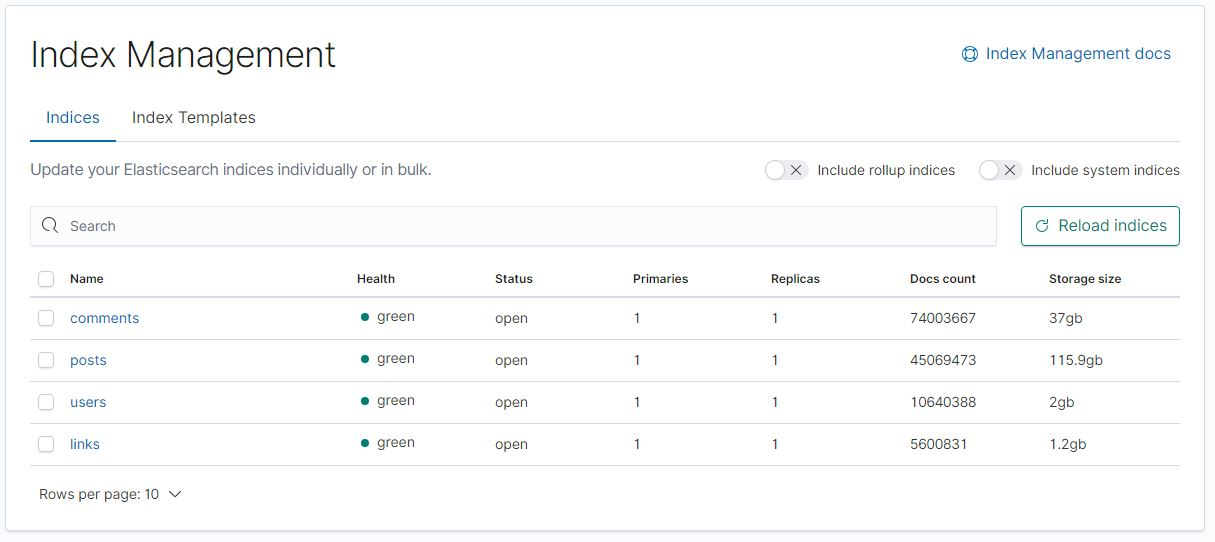
\includegraphics[width=15cm]{index_screenshot.JPG}
	\centering
	\caption{Summary of all documents indexed in the Elasticsearch cluster.}
	\label{index_summary}
\end{figure}

\begin{figure}[!h]
	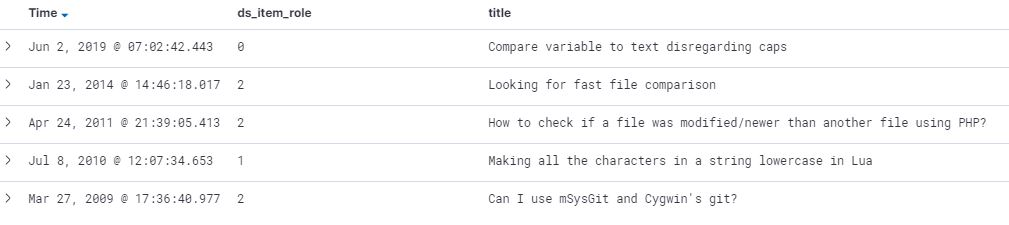
\includegraphics[width=15cm]{ds_item_group.JPG}
	\centering
	\caption{One dataset group displayed in the Kibana instance. The figure shows a master post (\textit{ds\_item\_role = 0}) with a corresponding duplicate (\textit{ds\_item\_role = 1}) and three similar posts (\textit{ds\_item\_role = 2}).}
	\label{ds_item_group}
\end{figure}


\begin{figure}[!h]
	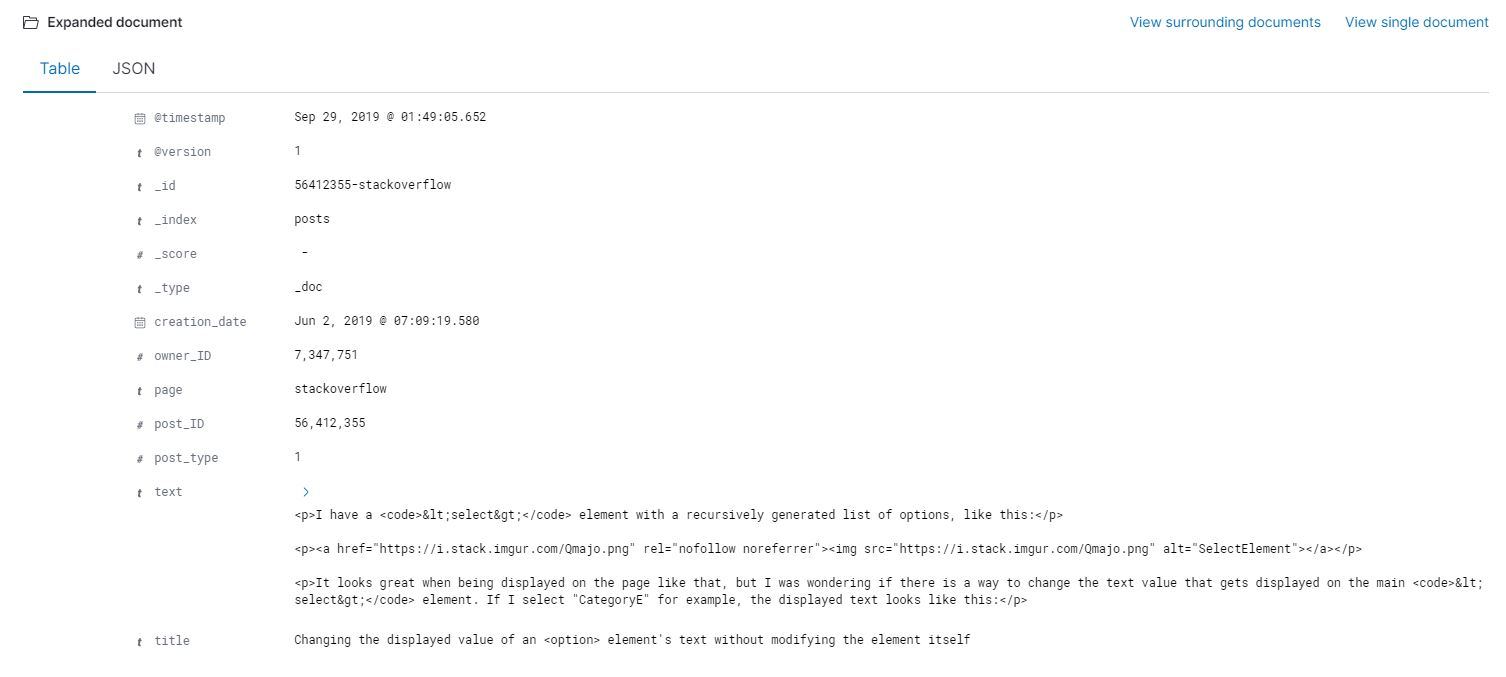
\includegraphics[width=15cm]{es_document_screenshot.JPG}
	\centering
	\caption{Expanded details of one document (post) displayed in the Kibana instance.}
	\label{es_document}
\end{figure}

\begin{figure}[!h]
	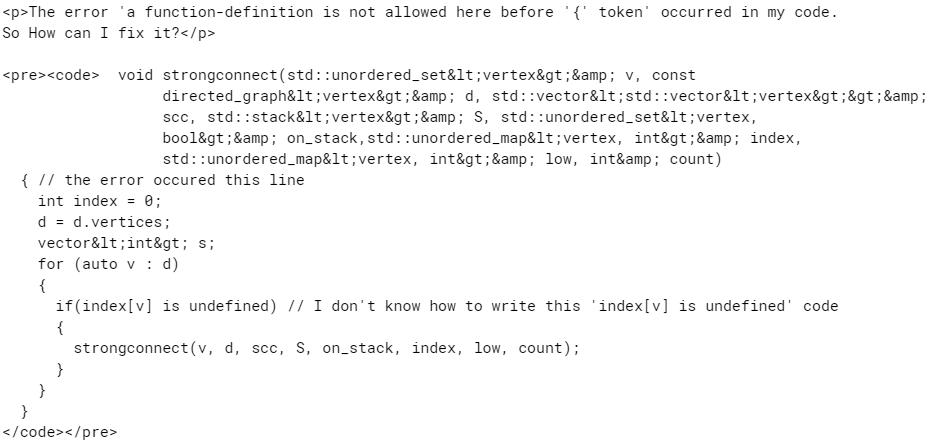
\includegraphics[width=15cm]{question_sample.png}
	\centering
	\caption{Example of an HTML body of one post.}
	\label{question_sample}
\end{figure}

\chapter{Demonstration Application}\label{demo_app}
\paragraph{}
We created a web application that allows us to browse and search in the Stackoverflow data using the Elasticsearch full-text queries. Furthermore, the application is ready for the integration of information retrieval techniques using the obtained vector representations of questions. In other words, the application will serve to demonstrate the benefits of this work, which is beyond the scope of this work.

\paragraph{}
In this appending, you can find screenshots (figures \ref{web_app_home} - \ref{question_2}) obtained from the application. Each screenshot is accompanied by a short caption with a description of the functionality. The purpose of the screenshots is to get an impression of how does the application work. A reader is not expected to read the text in the figures.

\begin{figure}[!h]
	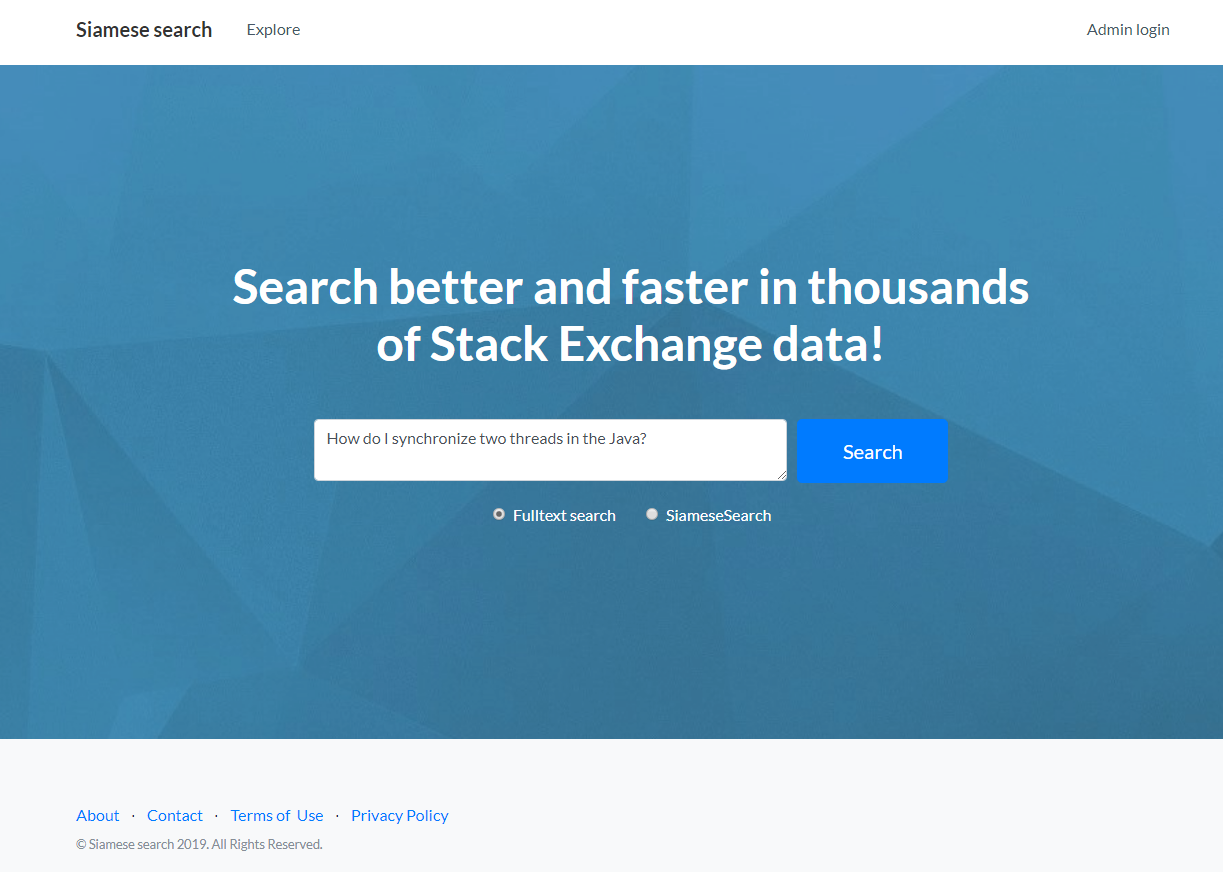
\includegraphics[width=19cm, angle=90]{web_app_home.PNG}
	\centering
	\caption{A homepage of the web application. In the middle of the screen, there is a text field for a query and a corresponding \textit{search} button. Users can select whether to use standard the full-text search or the improved search technique using our outcome. However, the latter is not implemented at the moment.}
	\label{web_app_home}
\end{figure}

\begin{figure}[!h]
	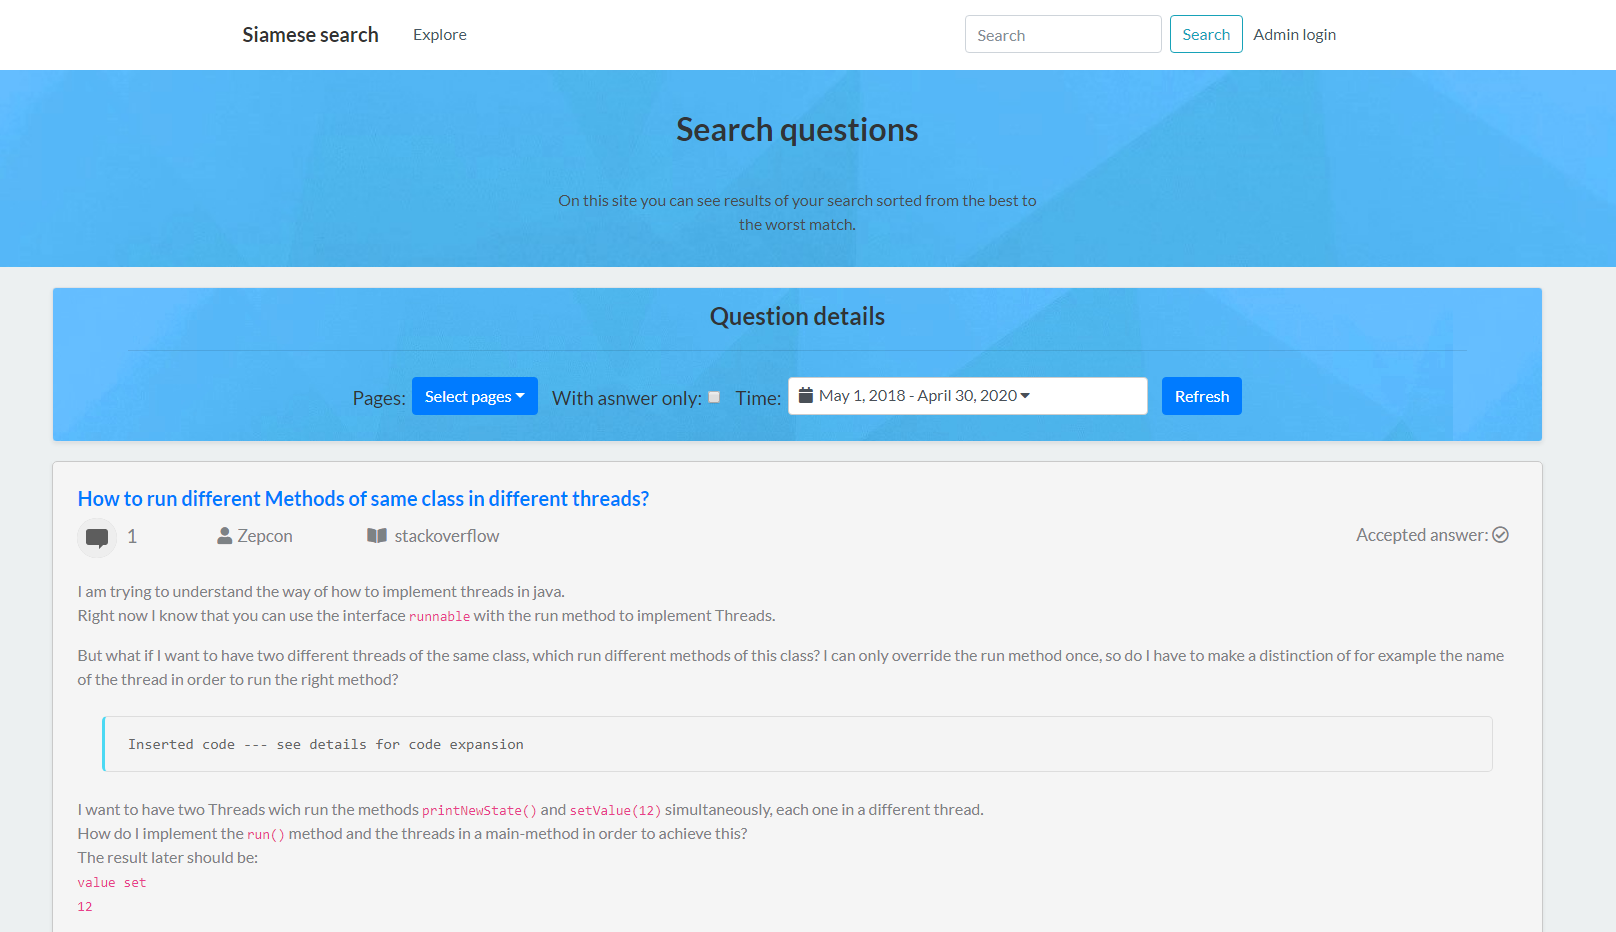
\includegraphics[width=20cm, angle=90]{search_res.PNG}
	\centering
	\caption{This figure shows a page with the results of the query displayed in figure \ref{web_app_home}. The page displays individual results with necessary information. Users can show details of the question by clicking the link in the title.}
	\label{search_res}
\end{figure}

\begin{figure}[!h]
	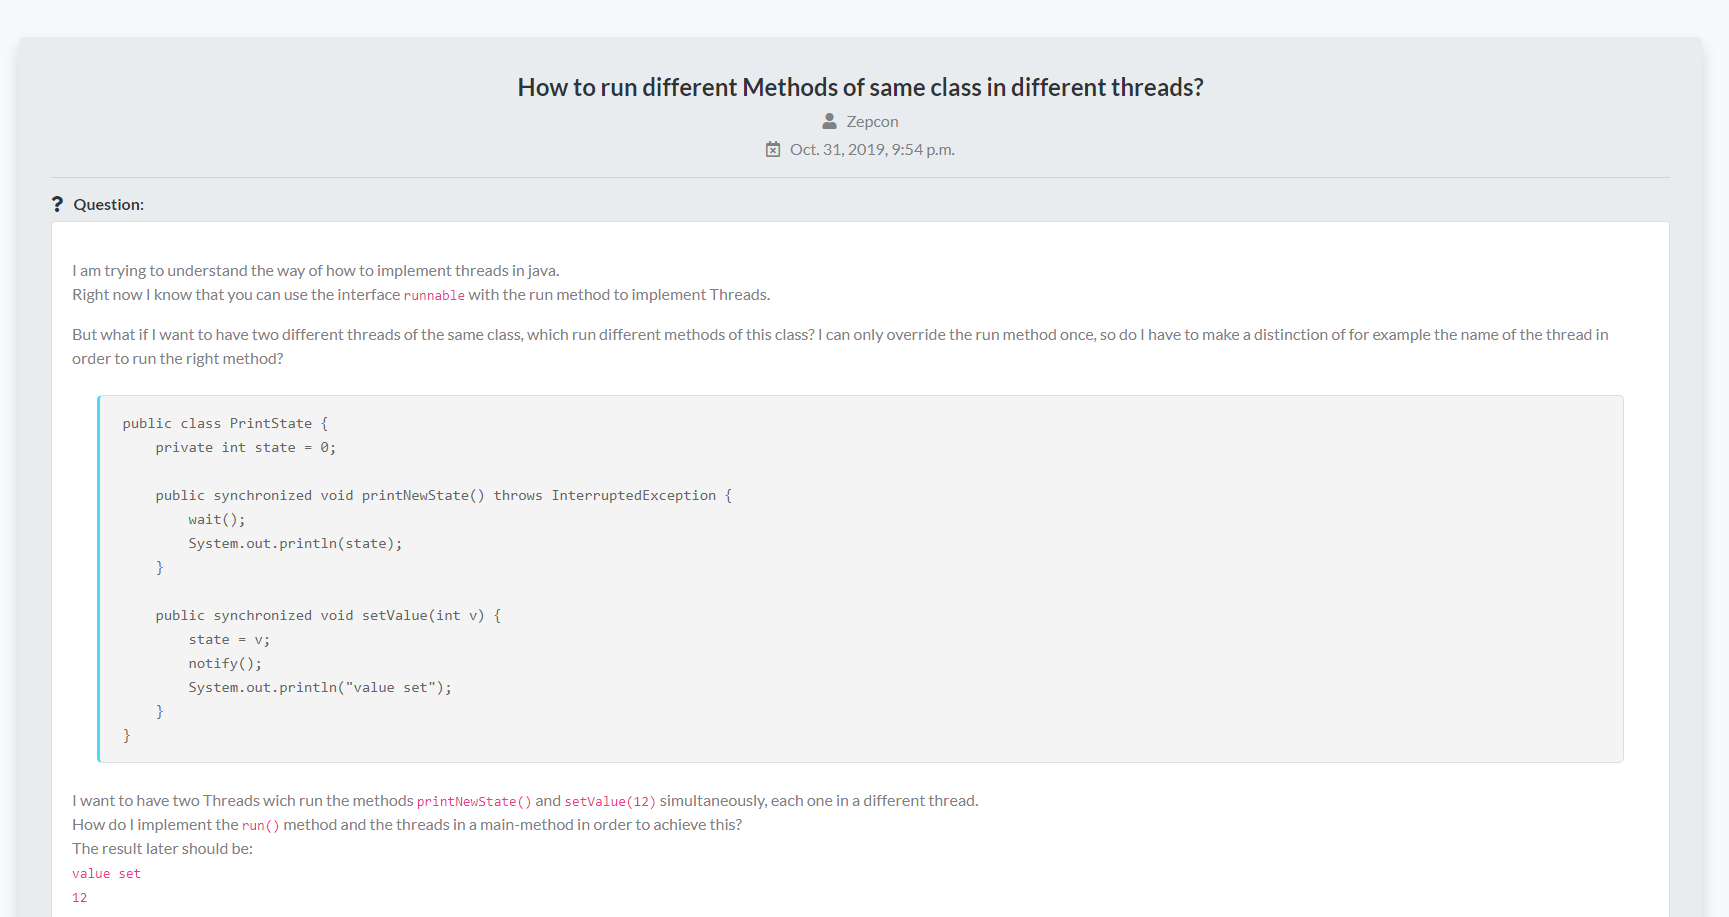
\includegraphics[width=20cm, angle=90]{question_1.PNG}
	\centering
	\caption{This figure shows a part of a page with details of the Stackoverflow question. On the top of the page, a title, author, and publish date is displayed. The question details are followed by expanded text and code snippet of the question.}
	\label{question_1}
\end{figure}

\begin{figure}[!h]
	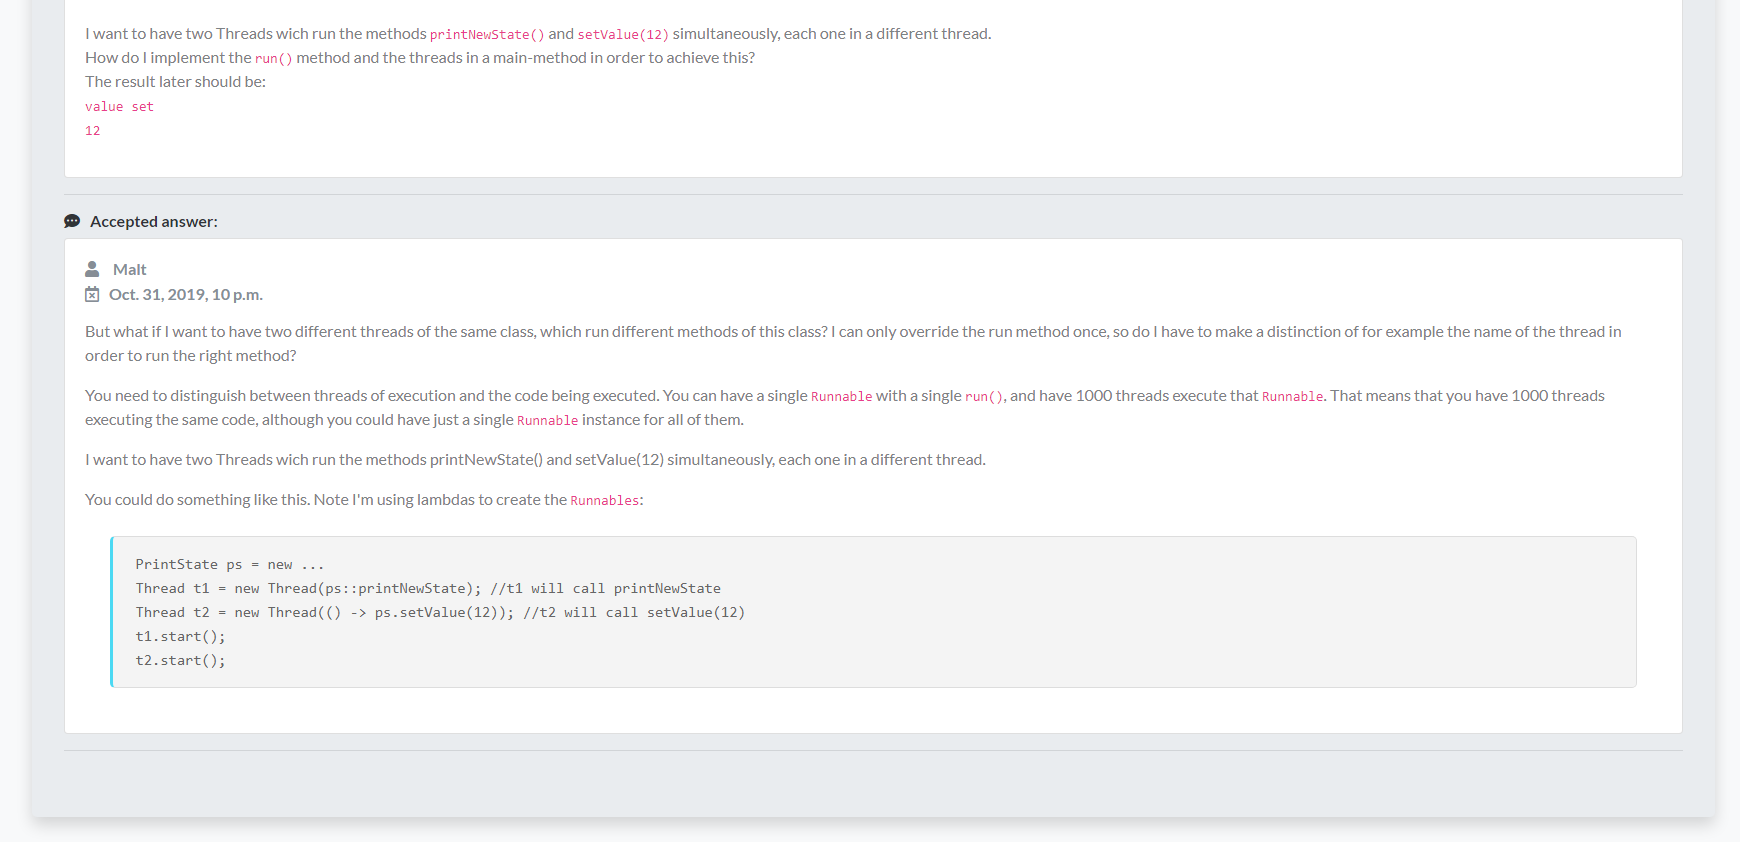
\includegraphics[width=20cm, angle=90]{question_2.PNG}
	\centering
	\caption{This figure follows the question details depicted in figure \ref{question_1}. In this part of the question detailed view, all answers and comments are displayed.}
	\label{question_2}
\end{figure}


\end{document}
